% Chapter 1
\chapter{Marco Teórico} % Main chapter title

\label{Cap_SDT} % For referencing the chapter elsewhere, use \ref{Chapter1} 

%----------------------------------------------------------------------------------------

% Define some commands to keep the formatting separated from the content 
\newcommand{\keyword}[1]{\textbf{#1}}
\newcommand{\tabhead}[1]{\textbf{#1}}
\newcommand{\code}[1]{\texttt{#1}}
\newcommand{\file}[1]{\texttt{\bfseries#1}}
\newcommand{\option}[1]{\texttt{\itshape#1}}

%----------------------------------------------------------------------------------------

\section{Teoría de Detección de Señales}

%Detectar ciertos estados en el mundo es importante para guiar nuestro comportamiento
Uno de los problemas más frecuentes a los que se enfrentan los organismos como sistemas inmersos en entornos variables que buscan optimizar su comportamiento, es la detección de estados o eventos específicos (\textbf{señales}) que de acuerdo a su experiencia y tras la definición de ciertas relaciones de contingencia, les proporcionen información relevante sobre el estado del mundo, las restricciones vigentes y la disponibilidad de eventos biológicamente importantes, \parencite{McNicol1}.\\

%Origen y expansión de la Teoría de Detección de Señales en la psicología y otras áreas
La Teoría de Detección de Señales (SDT, por sus siglas en inglés) aparece por primera vez en 1954 -como tantos otros avances científicos y tecnológicos motivados por las necesidades planteadas por la Segunda Guerra Mundial- en el contexto del estudio y desarrollo de radares para detectar señales eléctricas específicas \parencite{Peterson1954}. Muy poco tiempo después, los psicólogos John A. Swets y Wilson P. Tanner contribuyeron a la expansión de la teoría a un contexto psicológico, como un modelo para estudiar la percepción de los organismos, \parencite{Tanner1954, Swets1961}. Desde entonces, la SDT constituye uno de los modelos más estudiados, desarrollados y ampliamente aplicados en Psicología \parencite{Stainslaw1999}, extendiéndose desde su foco inicial en el estudio de la percepción \parencite{Rosenholtz2001, Pessoa2005, Wallis2007} hacia el estudio de cualquier fenómeno o escenario donde los organismos se enfrenten al problema de emitir -y guiar su comportamiento en función a- juicios de detección; por ejemplo, en materia de la emisión de diagnósticos clínicos \parencite{Grossberg1978, Swets2000, Boutis2010}, en el estudio de ciertas condiciones clínicas \parencite{Westermann2010, Bonnel2003, Brown1994, Naliboff1981}, en el estudio de la identificación visual de testigos \parencite{Gronlund2014, Wixted2014, Wixted2016} y un muy amplio \textit{etcétera} \parencite{Gordon1974, Nuechterlein1983, Harvey1992, Verghese2001}.\\ 

%La Teoría de Detección de señales como un modelo descriptivo para el problema de la detección que admite la importancia de la incertidumbre, como parte del entorno y como motor en el uso de sesgos de respuesta.
La SDT constituye un modelo estadístico que describe el problema al que se enfrentan los organismos inmersos en situaciones de detección en ambientes con incertidumbre, donde las \textit{señales} -los estímulos cuya ocurrencia interesa detectar- coexisten con \textit{ruido} -estímulos que no son la señal pero que pueden confundirse con esta-. Se trata de un modelo de decisión que entiende la detección como una tarea de elección, donde los organismos no responden simplemente con base en lo que perciben, sino que emiten el juicio de detección que les permita guiar su comportamiento de la manera mas óptima posible dada la información que poseen sobre su entorno y la evidencia presente, \parencite{Swets2000, Killeen2014}.\\

La generalizabilidad del modelo de la SDT al estudio de distintos fenómenos y tareas de detección es posible gracias a lo abstracto de sus elementos: la señal que interesa detectar puede ser desde un estímulo concreto -una luz o un tono- hasta la pertenencia a una categoría -una enfermedad o amenaza- y el ruido es simplemente todo elemento presente en el entorno de la tarea que no sea la señal, \parencite{Stainslaw1999, McNicol1}.\\ 

\subsection{Supuestos generales del modelo}

%La TDS distingue dos grandes factores en la emisión de un juicio o respuesta: La discriminabilidad y el sesgo.
La SDT funciona como una herramienta -o marco de análisis- para traducir el desempeño observado en tareas de detección en inferencias sobre la precisión con que la señal se distingue del ruido (la \textbf{discriminabilidad}) y la posible preferencia -o tendencia- del sistema detector a responder en favor o en contra de esta (el \textbf{sesgo}), \parencite{McNicol1}. Esta distinción entre la discriminabilidad de los estímulos comprometidos y el sesgo del sistema, como factores que interactúan en la emisión de juicios de detección, es una de las principales propiedades de la SDT \parencite{Swets1961} cuya importancia e implicaciones se discuten a continuación:\\

\textbf{1.- El papel de la Discriminabilidad: Siempre hay incertidumbre}\\

%Hay variabilidad en todos los estímulos implicados en las tareas de detección (en la señal y en los estímulos no-señal)
Se habla de la detección de señales como un problema de adaptación porque se asume que la variabilidad en la presentación y percepción de los estímulos en el ambiente merma la capacidad de los organismos de emitir juicios de detección que reflejen el estado del mundo con certeza, \parencite{Tanner1954}. Y dado que los \textit{estímulos-Señal} coexisten en el mundo con \textit{estímulos-Ruido}, saber qué tan salientes son las señales respecto del ruido es uno de los factores más importantes para determinar qué tan difícil es su detección para los organismos. En términos de la SDT, se habla de dicha dificultad como \textit{la discriminabilidad} de los estímulos comprometidos en la tarea.\\

De acuerdo con la SDT, la discriminabilidad constituye el primer gran componente en la emisión de juicios de detección óptimos que reflejen el verdadero estado del mundo y permitan al organismo actuar conforme a las consecuencias vigentes. La discriminabilidad suele explicarse en términos de:\\ %  1) la variabilidad intrínseca en la presentación de las señales y 2) el ruido con que ésta coexiste.\\

\underline{a) La Variabilidad en la Señal}\\

%Existe variabilidad en la forma en que percibimos los estímulos que nos rodean. Los sistemas sensoriales y perceptuales se comportan como instrumentos de medición (error de medida)
La noción de variabilidad ha sido uno de los principales motores para el desarrollo de modelos estadísticos en Psicología. Desde que Fechner extendió las ideas planteadas por Gauss sobre la incertidumbre contenida en toda medición -la idea de que toda medición realizada contiene el valor \textit{verdadero} de aquello que se quiere medir más un \textit{error} aleatorio que la carga de incertidumbre- al estudio de la percepción -conceptualizando nuestros sistemas sensoriales y perceptuales como instrumentos de medición que en cada observación perciben las cualidades verdaderas de los estímulos más un error- \parencite{Fechner, Gauss}, se sentaron las bases para el desarrollo de una amplia gama de modelos matemáticos y estadísticos en Psicofísica orientados a estudiar la relación entre las cualidades físicas -\textit{reales}- de los estímulos y la magnitud o intensidad con que se perciben psicológicamente \parencite{Link1994}.\\

%Variabilidad en la percepción de un mismo estímulo.
En el marco de la SDT, la variabilidad se considera una propiedad intrínseca de las señales a detectar bajo el supuesto de que ningún estímulo se percibe o se presenta de manera idéntica en cada exposición, \parencite{Tanner1954}. Por ejemplo, imaginemos los siguientes casos: \\

\begin{itemize}
\item Una persona es expuesta a un mismo tono con intensidad $X$ en cien ocasiones distintas y tras cada presentación, asigna un valor a la intensidad percibida. El valor reportado en cada ensayo será una mezcla entre el valor real del tono y un error aleatorio. Como se muestra en la Figura~\ref{fig:Senal_percepcion}, es muy probable que el valor percibido y reportado coincida con -o se acerque bastante a- su valor real (la media de la distribución, $\mu$, señalada con una línea vertical roja), pero también habrá ensayos en que aún tratándose del mismo estímulo, el valor percibido caiga por encima o por debajo de su valor real con cierta dispersión (las colas de la distribución). Este ejemplo catura la noción de que existe variabilidad en la forma en que se perciben los estímulos.\\

\item Un psicólogo aplica una prueba clínica \textit{A} para evaluar si su paciente tiene depresión. Por lo general, las pruebas clínicas arrojan un puntaje \textit{p} que, de acuerdo a su correspondencia con el rango de puntajes típicamente obtenidos por personas que tienen la condición, sugieren el diagnóstico a emitir. La Figura~\ref{fig:Senal_presentacion} presenta la idea central de este ejemplo: no todas las personas con depresión obtienen exactamente el mismo puntaje, sino que dentro de la serie de posibles puntajes a obtener en la prueba (todos los valores en el eje de las x), las personas con depresión suelen obtener resultados dentro de un rango específico con cierta probabilidad (la distribución azul), de tal suerte que hay puntajes que se asocian con dicha condición con mayor probabilidad (siendo la media de la distribución, $\mu$, señalada en rojo la más probable) que otros. Este ejemplo ilustra la idea de que hay variabilidad en la presentación de ciertos estímulos en el entorno.\\
\end{itemize}

\begin{figure}[th]
\centering
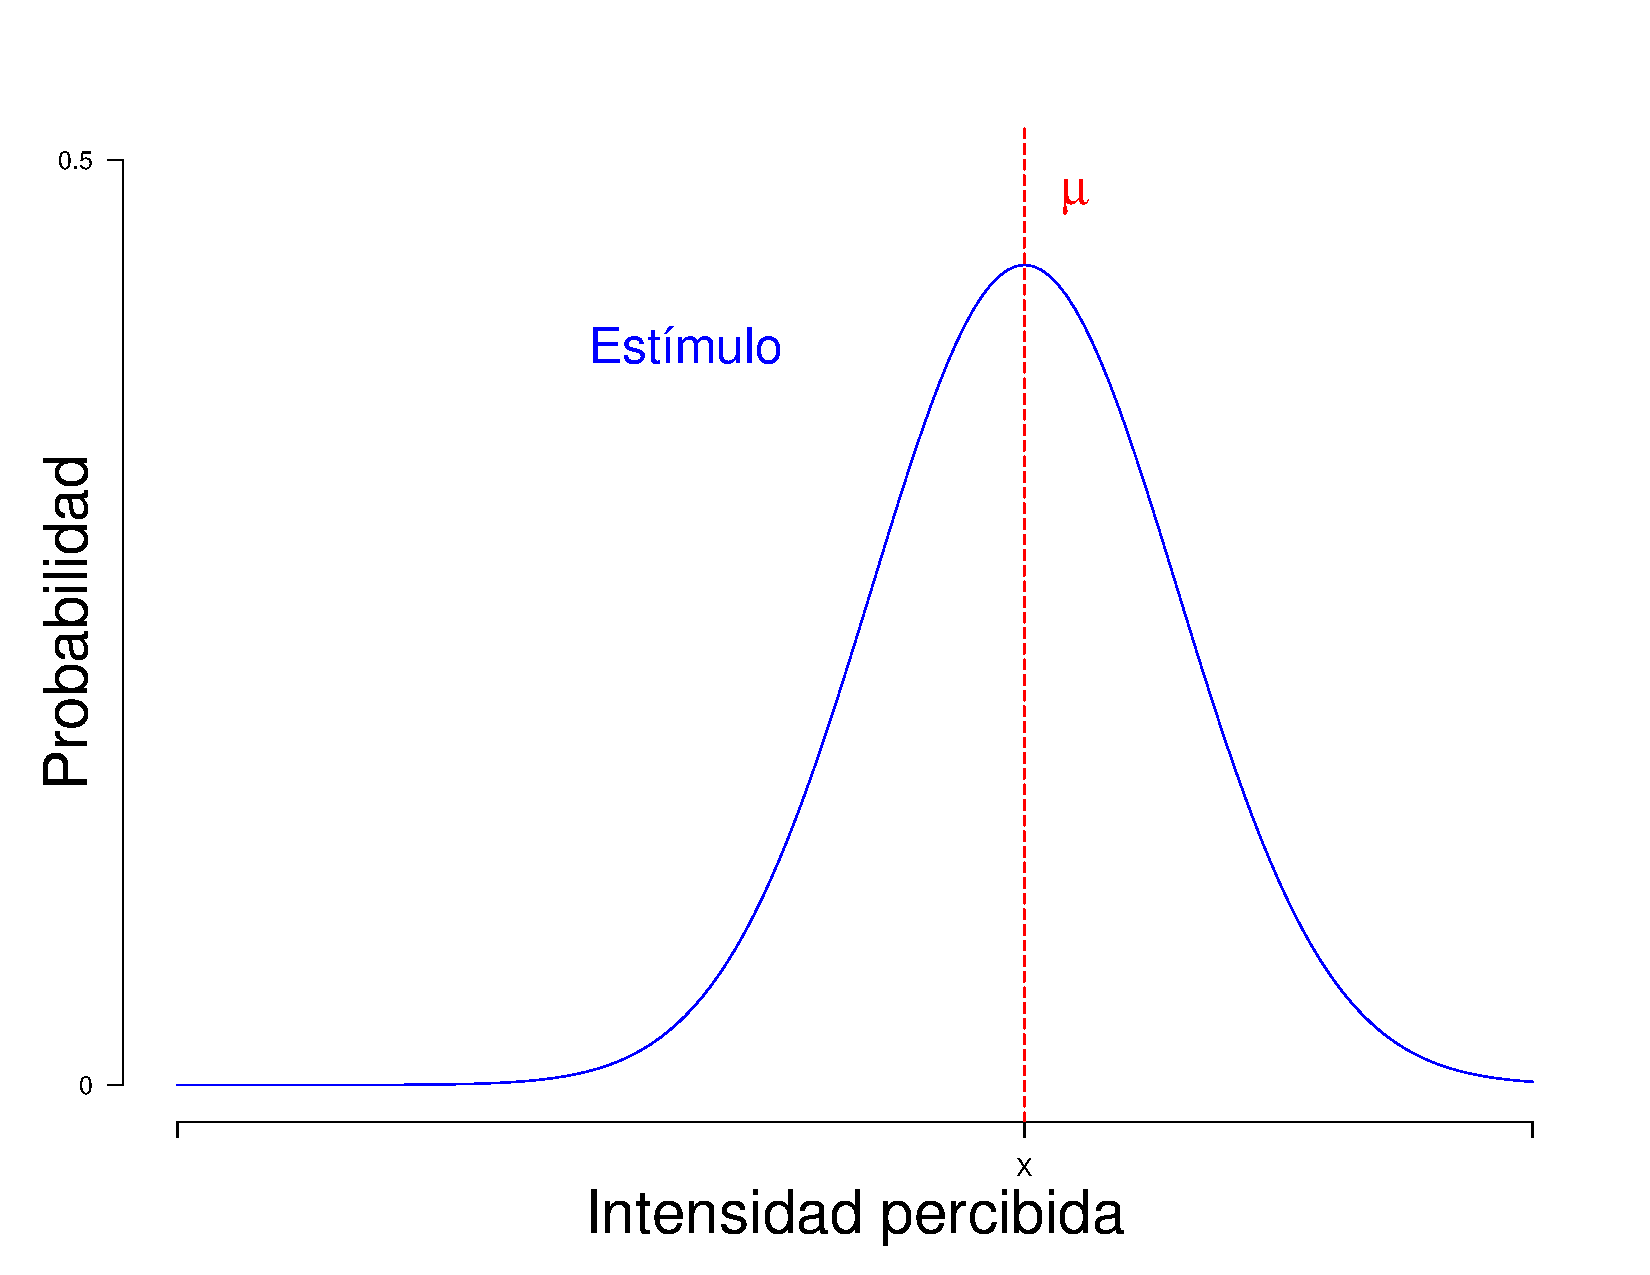
\includegraphics[width=0.70\textwidth]{Figures/Signal_Perception} 
%\decoRule
\caption[Variabilidad en la percepción de los estímulos]{Figura representativa de la variabilidad en la percepción de los estímulos. Si se presenta un mismo estímulo con intensidad x en repetidas ocasiones, es muy probable que el valor percibido se acerque a su valor real, (la media de la distribución, $\mu$) sin embargo y aunque con menor probabilidad, también habrán ocasiones en que sea percibido como más, o menos, intenso.}
\label{fig:Senal_percepcion}
\end{figure}


\begin{figure}[th]
\centering
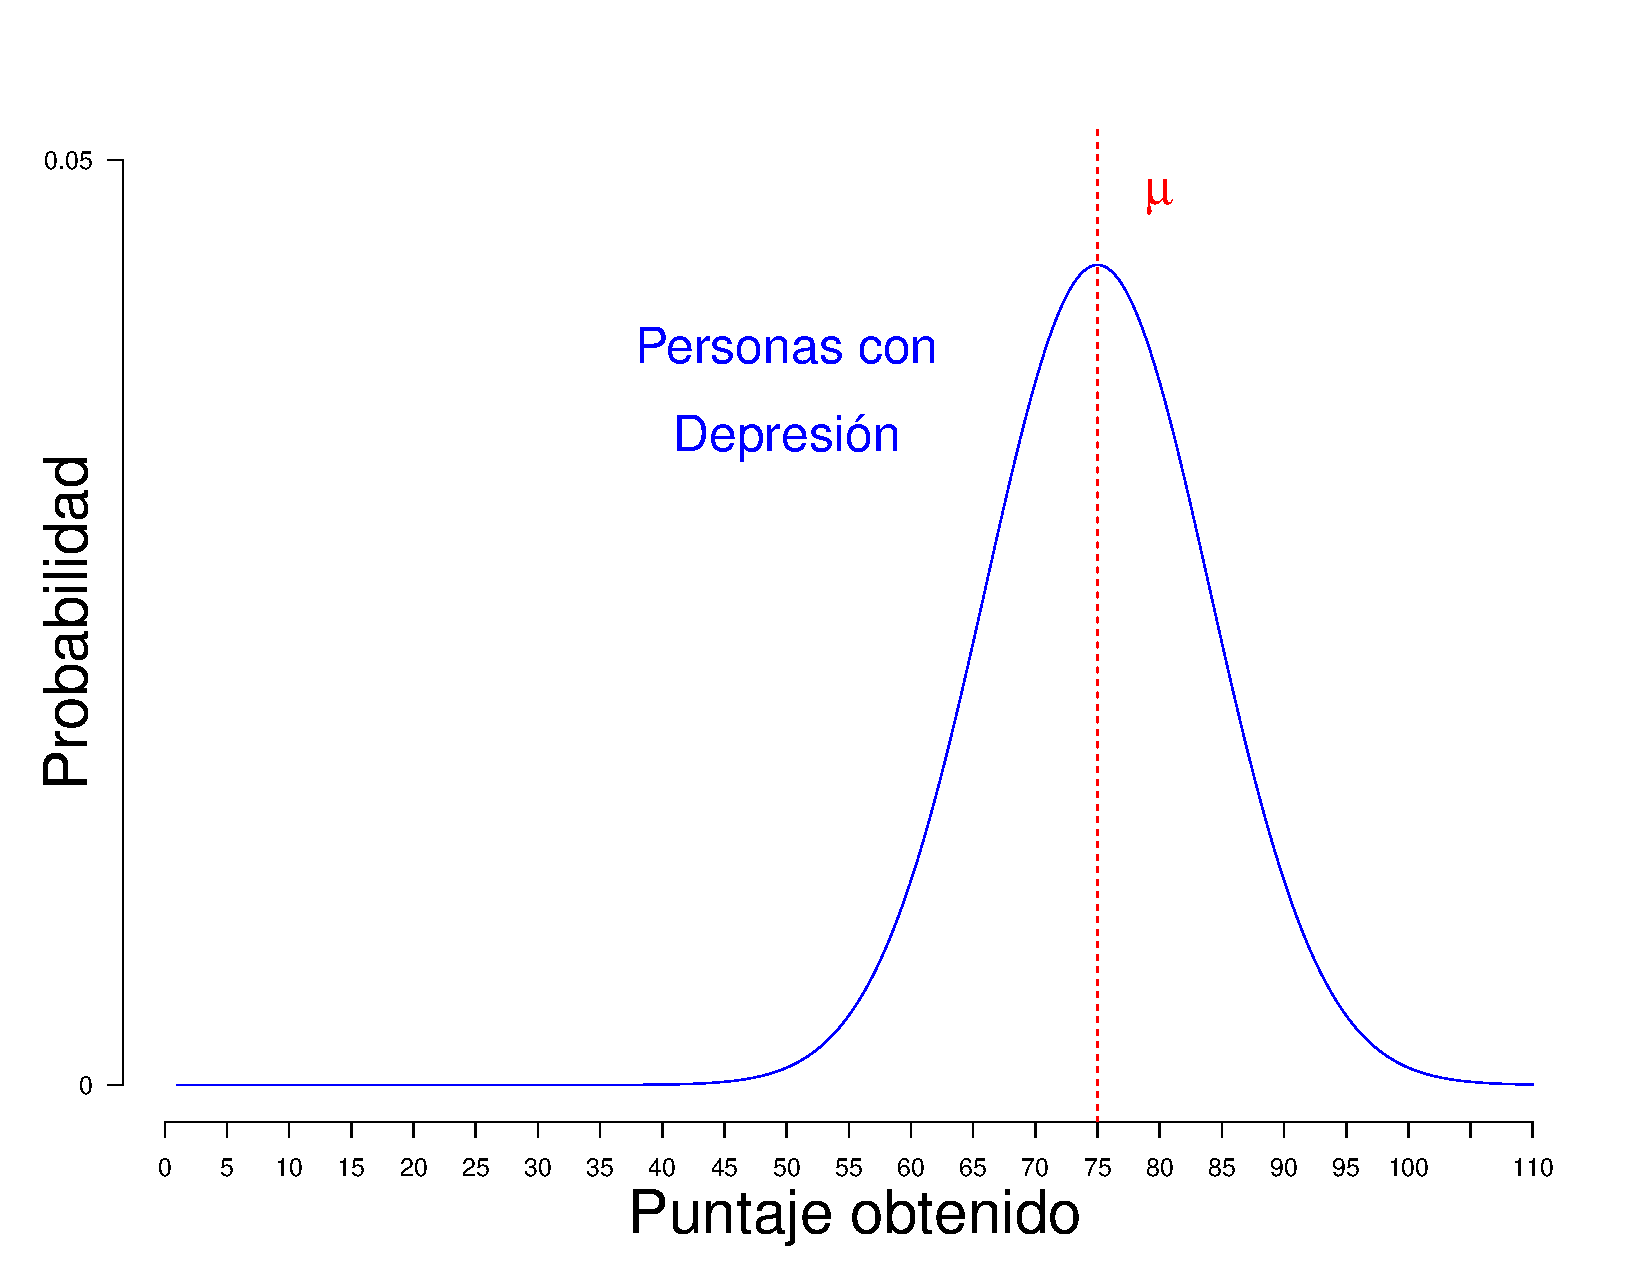
\includegraphics[width=0.70\textwidth]{Figures/Signal_Presentation} 
%\decoRule
\caption[Variabilidad en la presentación de los estímulos]{Figura representativa de la variabilidad en la presentación de los estímulos. Al aplicar una prueba clínica para detectar casos de Depresión, las personas con dicha condición pueden obtener puntajes dentro de un rango de valores con mayor o menor probabilidad al rededor de una media ($\mu$, señalado en rojo). Los valores presentados en la figura son arbitrarios.}
\label{fig:Senal_presentacion}
\end{figure}


En general, las Figuras~\ref{fig:Senal_percepcion} y \ref{fig:Senal_presentacion} representan un elemento fundamental para la forma en que la SDT concibe la detección de señales como un problema de adaptabilidad: la variabilidad es intrínseca a la percepción de los estímulos, ya sea porque nuestros sistemas sensoriales no los capturan igual en cada presentación, o porque los estímulos no se nos presentan exactamente de la misma forma en cada ocasión. Es decir, los estímulos en cuya detección están interesados los organismos (las señales) son intrínsecamente variables, \parencite{Tanner1954}.\\

    \underline{b) La variabilidad en el Entorno: Ruido}\\

%La señal coexiste con el ruido y puede llegar a confundirse con el mismo.
Además del hecho de que existe variabilidad implícita en las señales a detectar, es necesario tomar en cuenta que estas coexisten en el mundo con otros estímulos o estados que -dada su propia variabilidad- pueden llegar a producir evidencia similar y confundir el diagnóstico de detección emitido por los organismos implicados en la tarea, \parencite{Tanner1954}.\\

Retomando el ejemplo ilustrado en la Figura~\ref{fig:Senal_presentacion} sobre la variabilidad en los puntajes obtenidos en una prueba clínica por personas con una condición particular, la Figura~\ref{fig:Noise} presenta un segundo punto clave en la concepción de la detección de señales como un problema con incertidumbre: también existe variabilidad en los puntajes obtenidos por las personas que presentan la prueba sin tener dicha condición, de acuerdo a su propia distribución de probabilidad (la distribución agregada en color negro). Nótese que en la figura se presenta un pequeño rango de valores donde se traslapan las dos distribuciones y tomemos en cuenta que las pruebas clínicas se realizan para detectar -\textit{diagnosticar}- cierta condición -la señal- con base en el resultado obtenido por el paciente evaluado, ¿Cuál sería el diagnóstico pertinente para una persona que obtuvo un puntaje de 63 en la prueba, si dicha evidencia corresponde con lo que se espera observar tanto en pacientes con depresión como en los que no?. De acuerdo con la SDT, una forma ideal de resolver este conflicto -asumiendo que los organismos tienen un conocimiento perfecto sobre las distribuciones que subyacen a la presentación de los estímulos implicados en la tarea- es optar por el juicio de elección \texit{más probable} (es decir, el que tenga una densidad de probabilidad mayor en el punto representado por la evidencia evaluara), pero de cualquier forma, el problema persiste: existe incertidumbre en la tarea en tanto que la señal y el ruido pueden llegar a producir la misma evidencia, y los sistemas detectores no pueden tener certeza absoluta sobre el juicio de detección a emitir.\\ 

\begin{figure}[th]
\centering
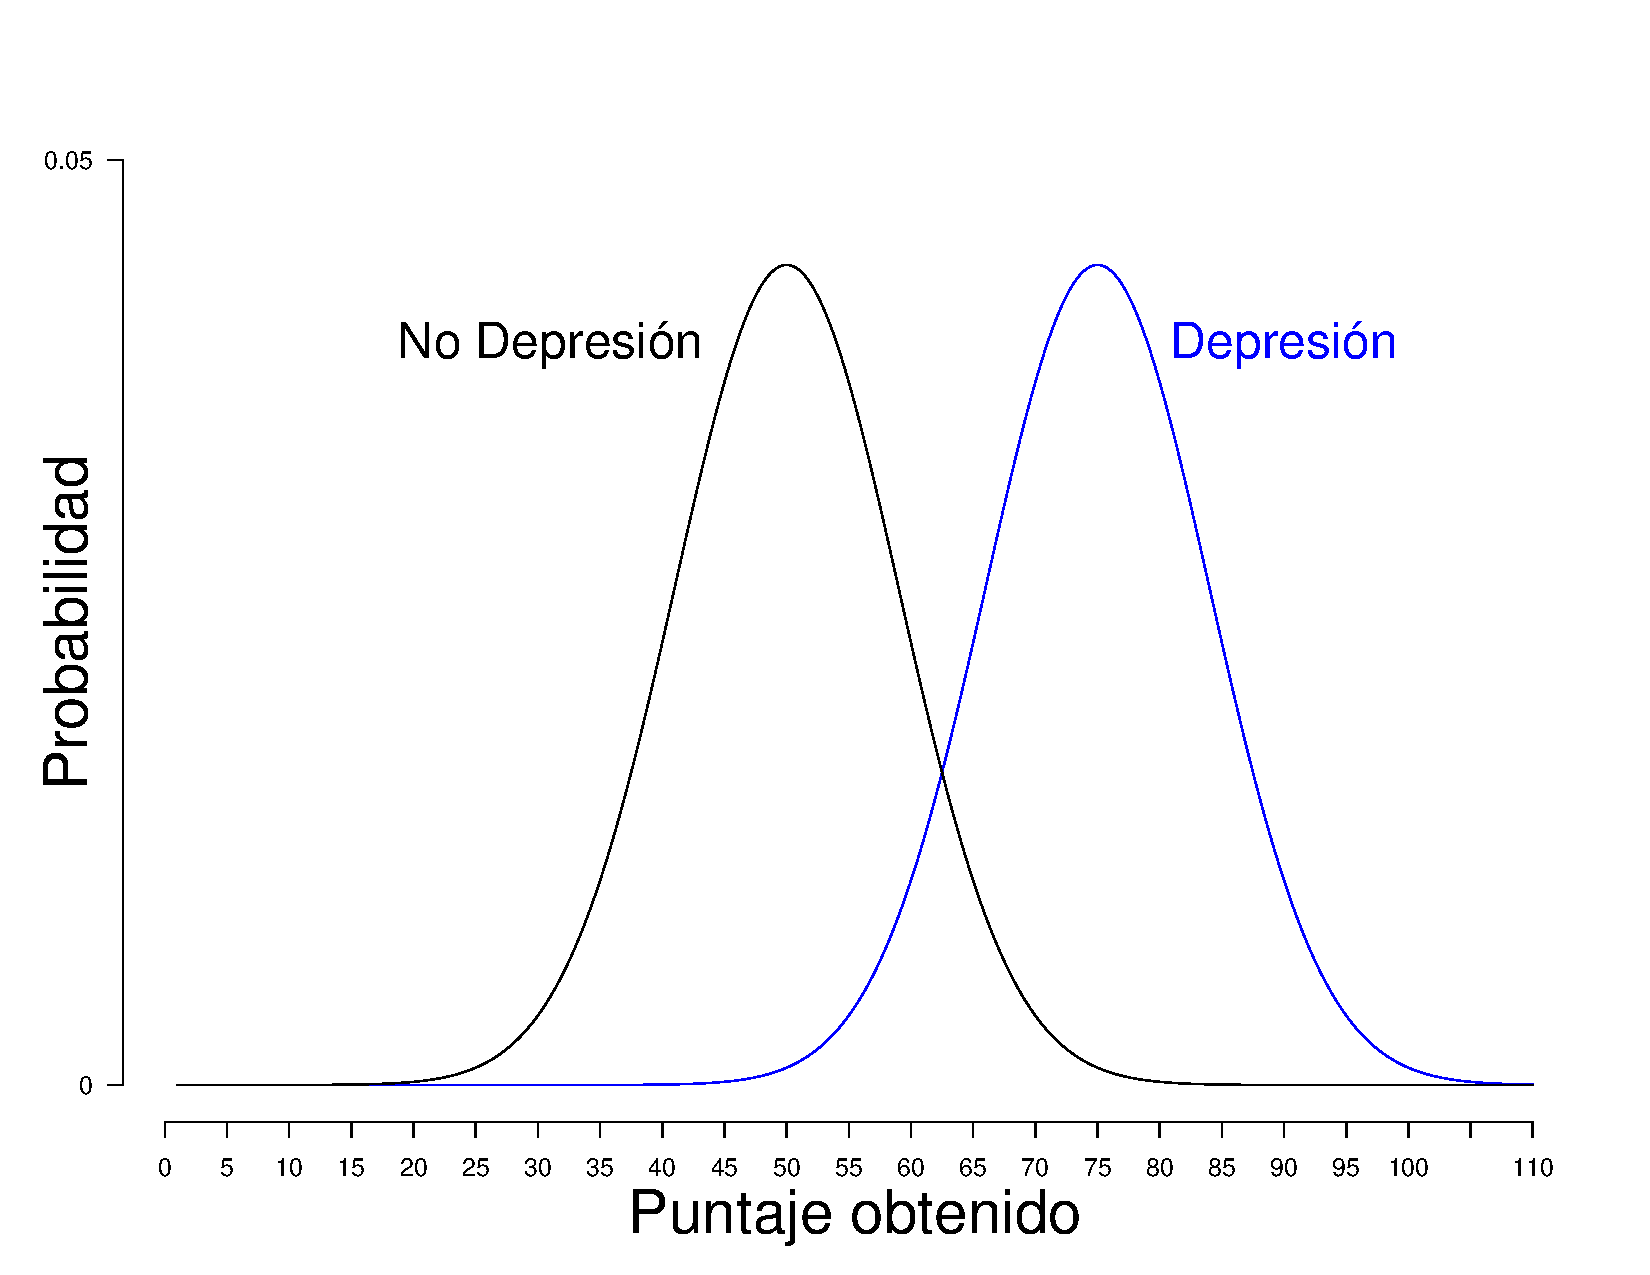
\includegraphics[width=0.70\textwidth]{Figures/Noise} 
%\decoRule
\caption[Variabilidad en la señal y en el ruido]{Como extensión del ejemplo acerca de la variabilidad en los puntajes a obtener en una prueba clínica por pacientes con depresión, además de la distribución que representa el rango de puntajes asociados con dicha condición (en azul), se añade una segunda distribución que representa el rango de puntajes observados en personas que realizan la misma prueba sin tener depresión (en negro). La Figura ilustra la noción de que los posibles estados del mundo -señal y ruido- se pueden presentar y percibir pueden confundirse entre sí, como se ilustra por el sobrelape entre las distribuciones. Los valores utilizados son arbitrarios.}
\label{fig:Noise}
\end{figure}

Al hablar de Discriminabilidad en tareas de detección bajo el marco de la SDT, se hace referencia a la probabilidad con que la señal y el ruido producen la misma evidencia (o bien, \textit{'¿qué tan probable es que la señal y el ruido se confundan?'}). En términos de la representación gráfica del problema con sus respectivas distribuciones de probabilidad, implica una evaluación de qué tan grande es el área de sobrelape, al considerar esta como un indicador fundamental de la incertidumbre contenida en la tarea (\textit{'¿Qué tan discriminable -diferente- es la señal respecto del ruido?'}).\\

La Figura~\ref{fig:Overlap} presenta dos figuras representativas que ilustran la relación entre la distancia entre las distribuciones de Ruido y Señal -y el área de sobrelape entre estas- y su interpretación en términos de la discriminabilidad de los estímulos contenidos en la tarea. En el panel superior (a), las distribuciones están muy separadas y el sobrelape entre estas es pequeño, sugiriendo un entorno con poca incertidumbre donde es muy poco probable encontrar evidencia que pueda confundir al organismo entre ambos estados del mundo -un entorno con \textit{discriminabilidad alta}-. Por otro lado, si las distribuciones están más juntas, como ocurre en el panel inferior (b), el sobrelape será más grande y habrá un mayor rango de valores de evidencia que se vinculen simultáneamente con ambos estados del mundo, ante los cuales el organismo no podría tener certeza sobre el juicio de detección correcto -un entorno con \textit{discriminabilidad baja}-.\\

\begin{figure}[th]
\centering
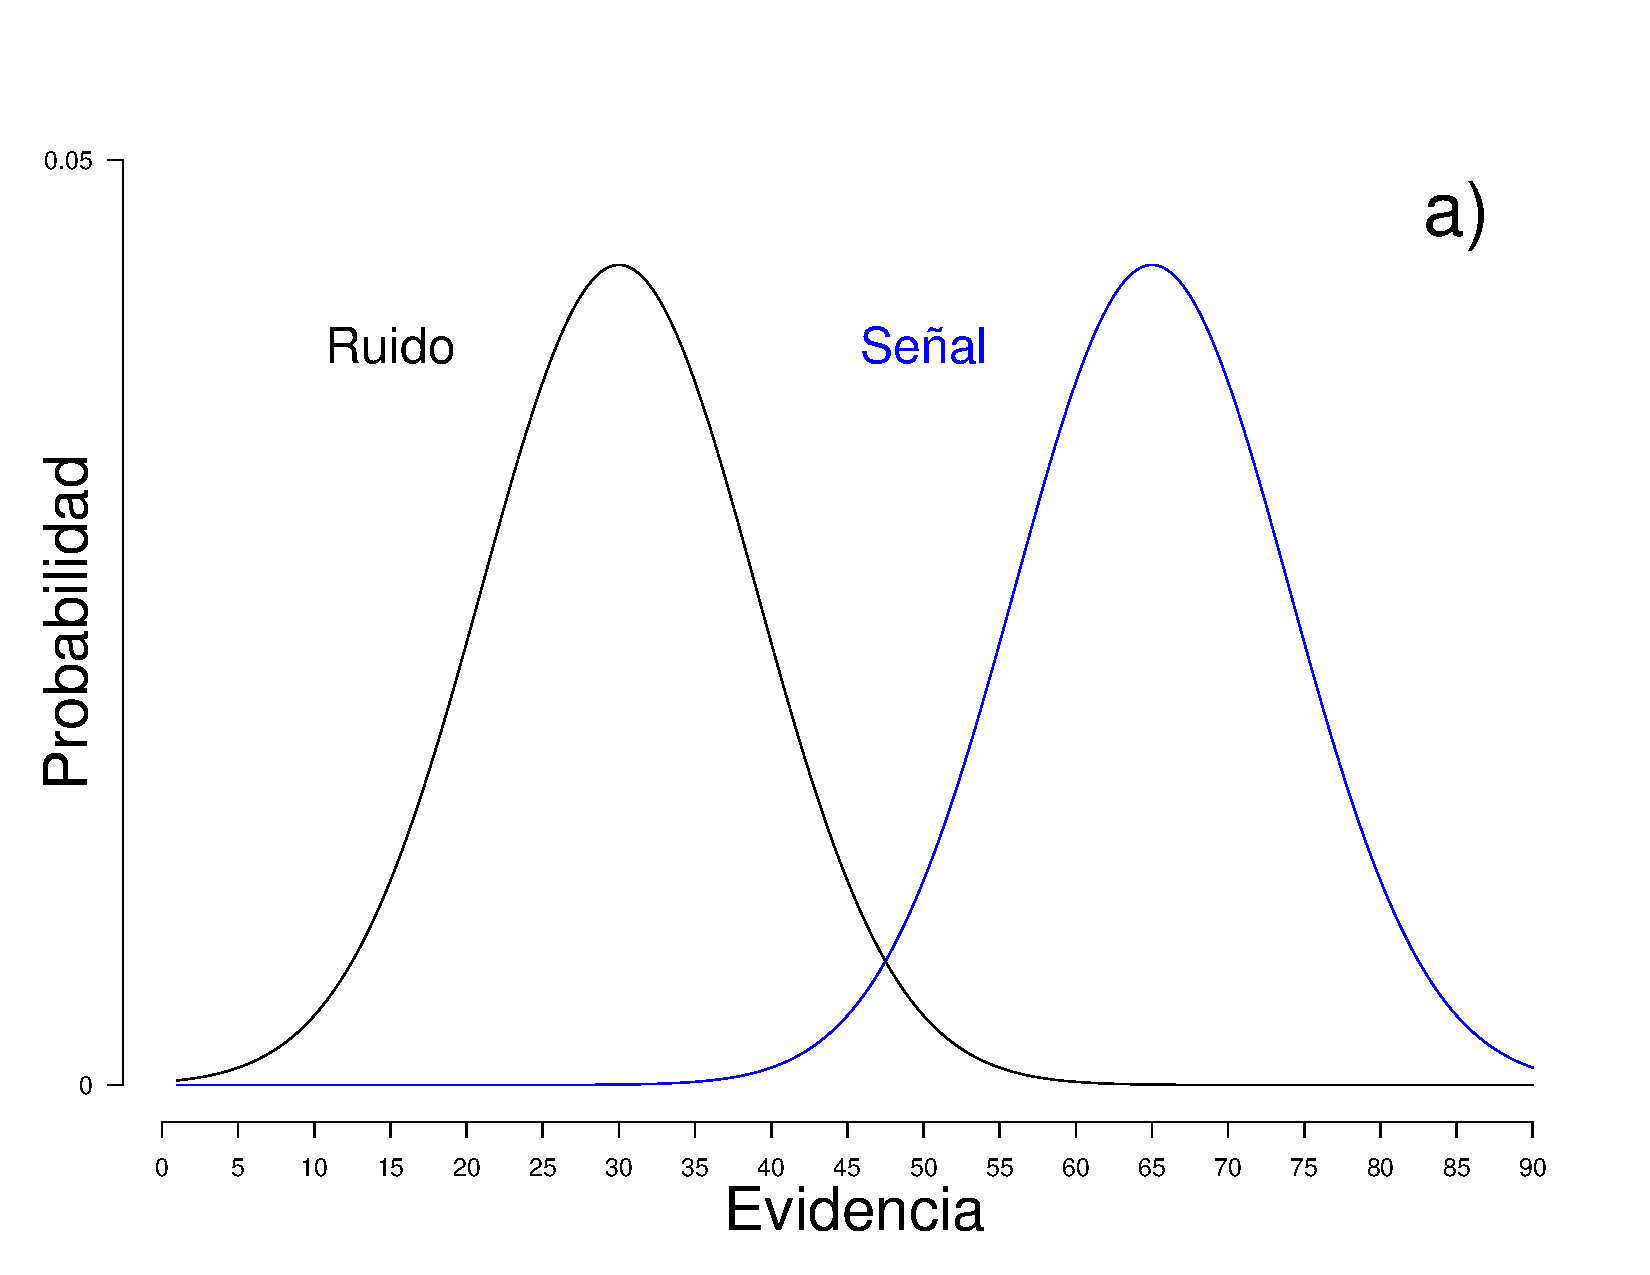
\includegraphics[width=0.55\textwidth]{Figures/Overlap_Small}\\ 
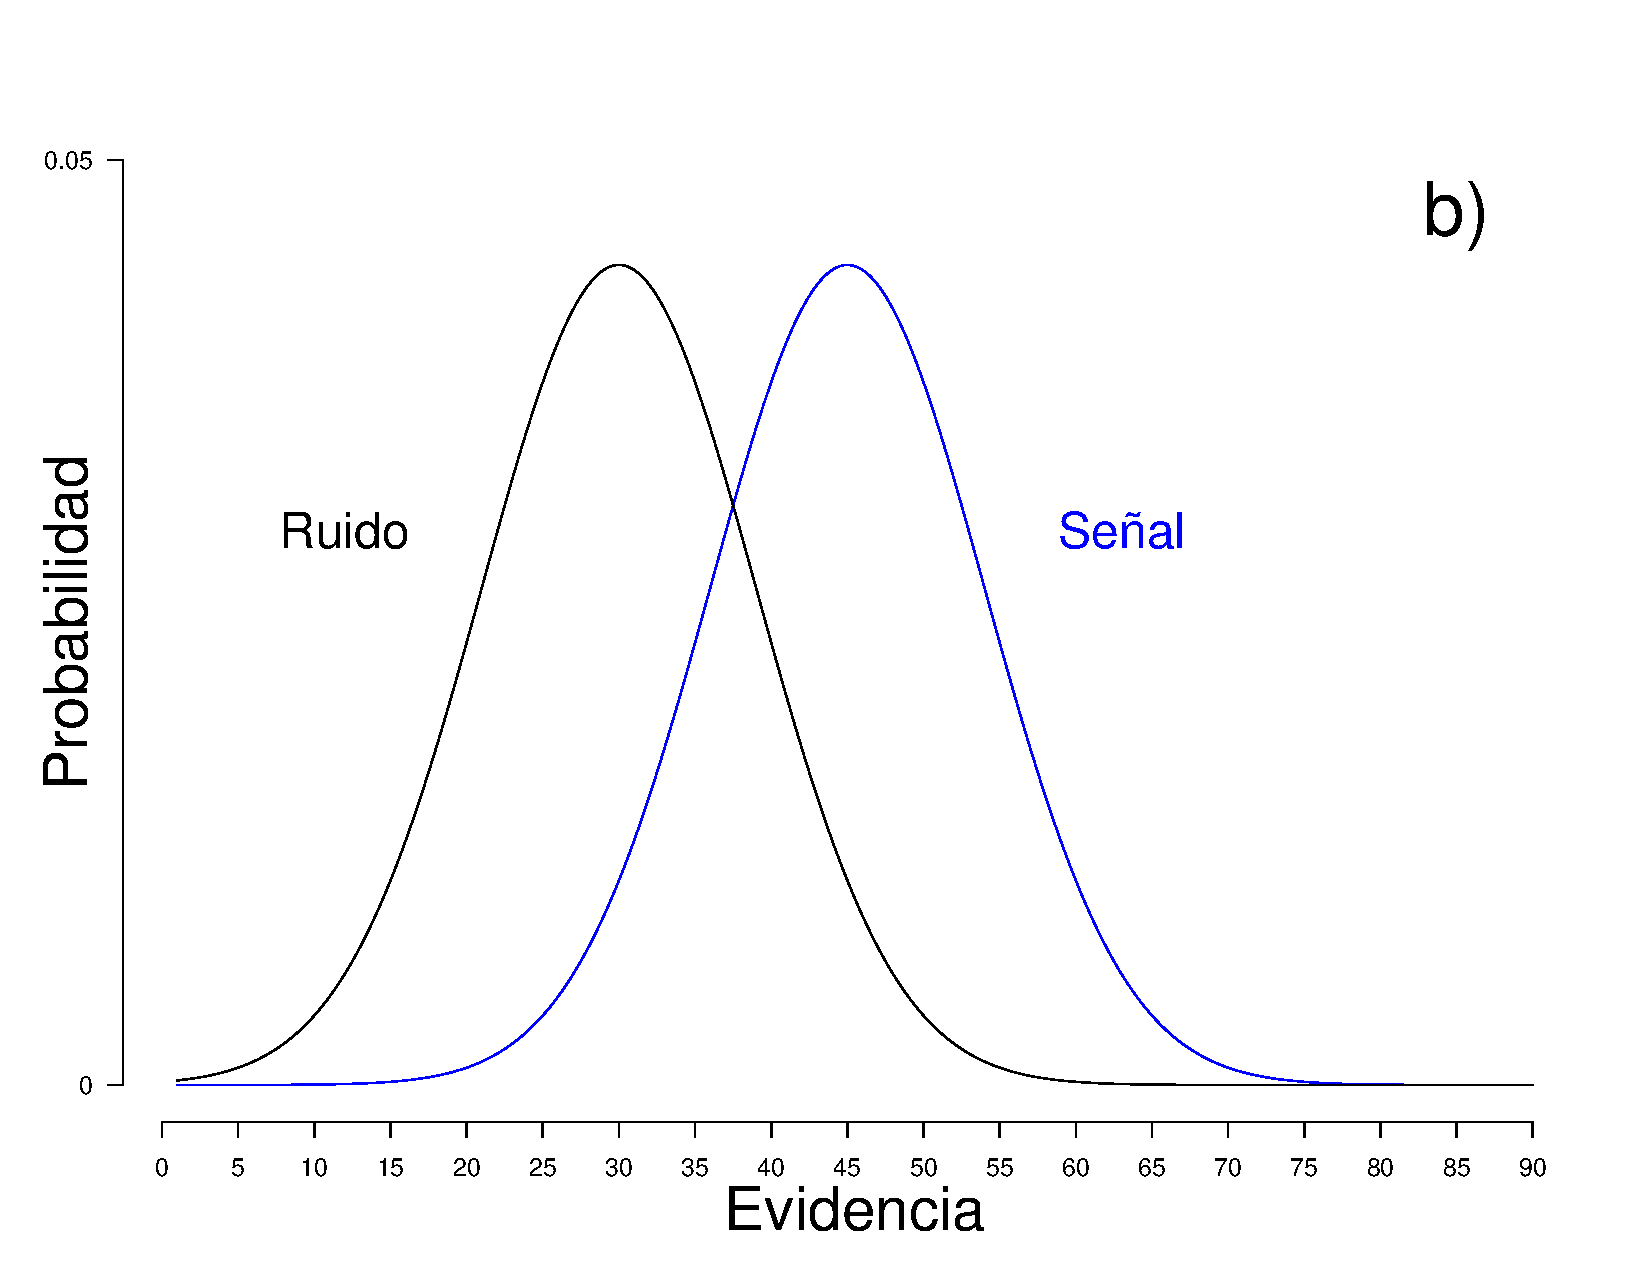
\includegraphics[width=0.55\textwidth]{Figures/Overlap_Big} 
%\decoRule
\caption[El sobrelape Ruido-señal como reflejo de la incertidumbre contenida en tareas de detección]{La distancia entre las distribuciones de ruido y señal determina la incertidumbre contenida en la tarea de detección al variar el área de sobrelape entre las mismas. En el panel a) se presenta un ejemplo donde al estar muy separadas las distribuciones, el sobrelape es pequeño y se asume poca incertidumbre. En el panel b) se muestra un segundo escenario donde las distribuciones están más cerca y comparten más evidencia en el área de sobrelape, describiendo una mayor incertidumbre.}
\label{fig:Overlap}
\end{figure}

La Discriminabilidad en una tarea de detección es producto de la variabilidad con que los posibles estados del mundo se presentan y perciben por los sistemas detectores. Es decir, depende tanto de las propiedades intrínsecas de los estímulos a evaluar -\textit{¿Qué tanto parecido tienen los estímulos con la señal y los estímulos sin esta?}- como de la precisión con que los sistemas detectores son capaces de discernir entre dichas instancias -\textit{¿Qué tan bueno es el organismo para distinguir una señal del ruido?}-, \parencite{Nevin1969}. Por ejemplo, no es lo mismo tratar de detectar una manzana entre un montón de naranjas que entre un montón de melocotones, (en general, esperaríamos que la tarea fuera más sencilla en el primer escenario al tener una mayor discriminabilidad); de la misma forma, la tarea de detectar si un instrumento musical está desafinado no es igual de difícil para un músico que para una persona sin educación musical.\\

  \textbf{2.- El papel del Sesgo: La detección es decisión}\\

La variabilidad en la presentación y percepción de los posibles estados del entorno -la presencia o ausencia de la señal- constituye el elemento base sobre el cual se desarrolla la SDT y que lleva a concebir la detección de señales como una tarea cargada de incertidumbre, donde los organismos no pueden confiar completamente en la evidencia que se les presenta para emitir un juicio de detección.\\

De acuerdo con la SDT, los organismos compensan la incertidumbre contenida en las tareas de detección con la información que poseen sobre el entorno que, en términos generales, puede ser de dos tipos: 1) información probabilística e 2) información sobre las consecuencias comprometidas, \parencite{Nevin1969}.\\

Como ejemplo, tomemos el caso de un médico que trata de decidir si los resultados obtenidos en cierta prueba clínica son evidencia suficiente para diagnosticar una enfermedad \textit{X} a un paciente \textit{Y}. La evidencia con la que el médico cuenta es imprecisa: toda prueba clínica tiene un margen de error y su lectura debe complementarse con información extraída de la historia clínica del paciente; el médico debe juzgar la evidencia en función de toda la información de la que dispone: \textit{¿Qué tan confiable es la prueba?} o \textit{¿Cuál es su tasa de aciertos y errores?}; \textit{¿Qué tan común es la enfermedad cuya presencia se intenta determinar?} y \textit{¿Qué tan probable es que el paciente Y tenga la enfermedad X?}; de acuerdo con su historia clínica, \textit{¿Qué tanto correlacionan sus características con los factores de riesgo asociados a la enfermedad?} y \textit{¿Qué tanto afecta eso la probabilidad de que Y tenga la enfermedad X?}. Y aún ponderando toda esta información, el problema no termina aquí. La información probabilística permite hacer inferencias sobre cuál es la conclusión más \textit{probable}, pero sigue sin haber certeza sobre el diagnóstico. Para optimizar su comportamiento y tomar la mejor decisión posible, el médico también debe tomar en consideración la información que posee sobre las consecuencias asociadas a cada escenario posible: a) Si el paciente tiene la enfermedad y el médico la detecta acertadamente, podrá tratarse a tiempo; b) Si tiene la enfermedad y el médico falla en detectarla, podría poner en riesgo su vida; c) Si no tiene la enfermedad y el médico le dice que sí, se gastarán recursos innecesarios en solucionar un problema que no existe, corriendo el riesgo de que el tratamiento le haga daño y d) Si no tiene la enfermedad y el médico decide no darle el diagnóstico, todo permanecerá igual. La tarea del médico es mucho más compleja de lo que parecía en un principio, puesto que no se limita a la lectura de la prueba clínica, sino que tiene que ponderar lo que sugieren los resultados de la misma con toda la información que posee sobre la probabilidad de las interpretaciones posibles y las consecuencias comprometidas.\\

De acuerdo con la correspondencia entre el \textit{estado real del mundo} -la presencia o ausencia de la señal- y el juicio emitido por el sistema detector, la SDT distingue entre dos tipos de aciertos y errores, presentados en la matriz de contingencia presentada en la Figura~\ref{fig:Mat_Output}. Cuando la señal está presente el organismo puede detectarla adecuadamente (\textbf{Hit}) o dejarla pasar (\textbf{Omisión}); y si por el contrario, la señal no está presente, el organismo puede acertar al diagnosticar su ausencia (\textbf{Rechazo correcto}) o confundir el ruido con la señal, (\textbf{Falsa Alarma}).\\

\begin{figure}[th]
\centering
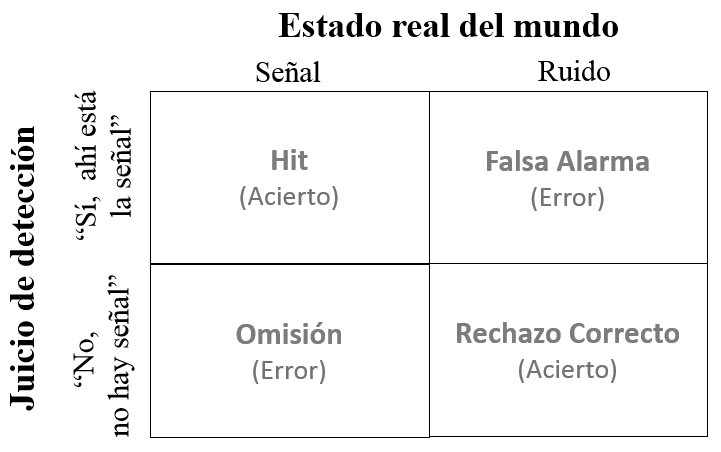
\includegraphics[width=0.60\textwidth]{Figures/Matriz_Outputs} 
%\decoRule
\caption[Matriz de contingencia con los posibles Resultados en una Tarea de Detección]{Los cuatro posibles resultados a encontrar de acuerdo con la SDT en función de la correspondencia que existe entre los juicios emitidos por los organismos y el estado real del mundo.}
\label{fig:Mat_Output}
\end{figure}

La SDT asume que con base en la información de la que dispone sobre la estructura de la tarea, el organismo fija un criterio de elección para determinar a partir de cuánta evidencia va a juzgar la presencia de la señal dado lo que sabe sobre la probabilidad con que ésta ocurre y las consecuencias comprometidas con su detección, \parencite{Tanner1954, Swets1961, Nevin1969}. En términos de la representación gráfica del modelo, implica que sobre el eje de la evidencia se sitúa una línea vertical  que atraviesa ambas distribuciones (como se ilustra en la Figura~\ref{fig:Graf_Outputs} con una línea roja), y que va a funcionar como regla de elección para definir a partir de cuánta evidencia el organismo emitirá juicios de detección en favor de la señal.\\

\begin{figure}[th]
\centering
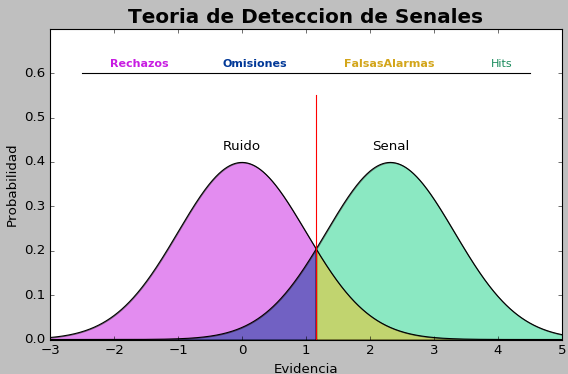
\includegraphics[width=0.90\textwidth]{Figures/Graficador_Tasas} 
%\decoRule
\caption[Representación gráfica de los posibles Resultados en una Tarea de Detección]{Representación gráfica del problema de detección de señales de acuerdo con la SDT: existen dos distribuciones de probabilidad que describen la forma en que la señal y el ruido se presentan en el entorno, que presentan un traslape que refleja la incertidumbre contenida en la tarea. El organismo enfrenta la variabilidad fijando un criterio de elección (la línea roja) para determinar a partir de cuánta evidencia juzgará la presencia de la señal, determinando la probabilidad de obtener los distintos tipos de acierto y error (señalados en la figura con distintos colores).}
\label{fig:Graf_Outputs}
\end{figure}

La Figura~\ref{fig:Graf_Outputs} presenta la forma final en que se representan los problemas de detección de señales bajo el marco de la SDT: Se tienen dos distribuciones de probabilidad que representan la variabilidad con que la señal y el ruido ocurren en el ambiente, \parencite{Tanner1954} y una línea roja que señala el criterio que el agente detector va a utilizar para determinar cuándo emitir un juicio de detección. Como se ilustra en la figura con distintos colores, la localización del criterio de elección determina la probabilidad con que, de acuerdo a la cercanía de las distribuciones, se esperaría incurrir en cada uno de los cuatro resultados expuestos en la matriz de contingencia de la figura~\ref{fig:Mat_Output}.\\

En función a la estructura de la tarea y al conocimiento que los organismo tengan sobre ella, es posible que se desarrolle un \textit{sesgo} que favorezca la emisión de un juicio de detección particular, \parencite{Nevin1969}. Se asume que la localización del criterio sobre el eje de evidencia es un reflejo del mismo, siendo que su magnitud y dirección depende de dos grandes factores:\\

      \underline{a) Los errores cuestan y los aciertos pagan: Matrices de pago}\\

La variabilidad asociada a la percepción de los estímulos en el ambiente abre la posibilidad de que los sistemas involucrados en tareas de detección cometan errores. Tomando en cuenta que las situaciones de detección se consideran importantes para la adaptabilidad de los organismos en tanto que la detección de ciertas señales les permite guiar su conducta en términos de las relaciones de contingencia anunciadas, acertar o errar en la emisión de un juicio de detección trae consigo consecuencias importantes. Es decir, los aciertos pagan y los errores cuestan, y más aún, cada tipo de acierto y error repercute de manera diferente.\\

Imaginemos el caso de un animal indefenso -un conejo- que tiene que decidir tan rápido como pueda si el sonido que acaba de escuchar en la maleza corresponde, o no, con el de un depredador. La penalización asociada con cometer una falsa alarma -un gasto innecesario de energía al correr para nada- es sustancialmente diferente a el precio que tendría que pagar por incurrir en una omisión -¡la muerte!-. Dadas las consecuencias en juego, es muy probable que el conejo decida actuar en consecuencia de un juicio de detección afirmativo (\textit{'¡Sí, es un depredador!'}) y correr por su vida, aún ante niveles de evidencia muy bajos.\\

\begin{figure}[th]
\centering
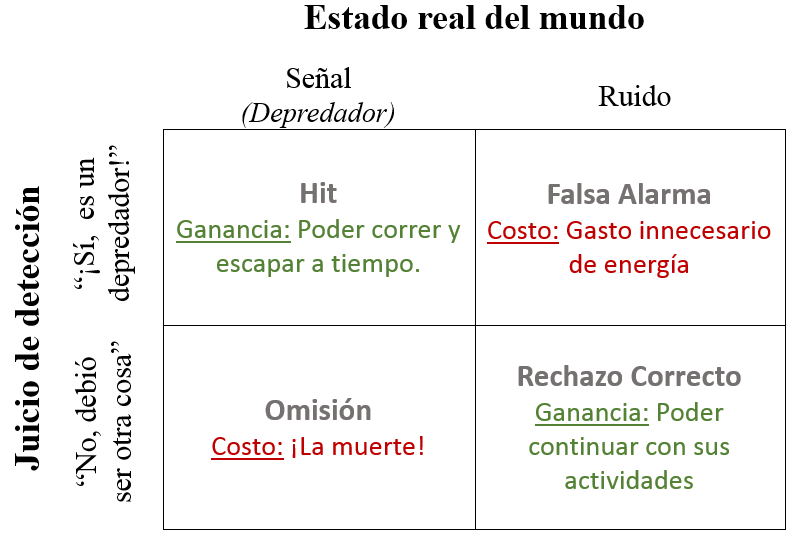
\includegraphics[width=0.60\textwidth]{Figures/Matriz_Pagos} 
%\decoRule
\caption[Ejemplo de Matriz de Pagos]{Se presenta como ejemplo la matriz de pagos que ilustra los costos y ganancias comprometidos en la tarea de detectar la presencia de un depredador, en función a la correspondencia entre el juicio elegido y el estado verdadero del mundo.}
\label{fig:Mat_Pagos}
\end{figure}

La figura~\ref{fig:Mat_Pagos} presenta lo que en los modelos clásicos de decisión se conoce como \textit{Matriz de Pagos} y que se utiliza para señalar, de acuerdo a una matriz de contingencia, los costos y ganancias asociados con los resultados a obtener en tareas de detección. De acuerdo con la SDT, los organismos toman en cuenta esta información para definir la localización de su criterio de elección. En otras palabras, ya que los organismos no pueden tener certeza absoluta sobre el juicios de detección a emitir, la evidencia es juzgada en función a un criterio de elección que toma en cuenta las consecuencias comprometidas para guiar su comportamiento de manera óptima, \parencite{Killeen2014}.\\

      \underline{b) Estimados de Probabilidad}\\

Los organismos involucrados en cualquier tarea de detección tienen alguna expectativa respecto de la probabilidad con que las señales de interés ocurren en el mundo. Es decir, ya sea como resultado de su experiencia directa o porque es información que les ha sido proporcionada de manera externa, \parencite{Nevin1969} los agentes detectores tienen alguna idea o conocimiento sobre la estructura probabilística de la tarea, en dos sentidos: 

\begin{itemize}
\item \textsl{Un estimado prior.} Con independencia de cuál sea la evidencia evaluada de manera inmediata,\textit{¿Qué tan probable es encontrar la señal en esta situación particular?}\\

Si los organismos se encuentran en un entorno donde saben que es prácticamente imposible encontrar la señal, es muy probable que decidan descartar la evidencia que se les presente aún si esta correlaciona con lo que se esperaría de una señal. Recordemos el ejemplo planteado con anterioridad sobre querer determinar la edad de una persona al hablar con ella por teléfono: si la llamada fue hecha a un despacho de abogados -o cualquier otro escenario donde se piense que es muy poco probable encontrar a un niño-, aún si la persona al otro lado del teléfono tiene una voz muy aguda, es muy poco probable que su interlocutor piense \textit{'Oh, estoy hablando con un niño'}.\\

\item \textsl{La verosimilitud.} Dado lo que se sabe sobre cómo se presentan ciertos estímulos en el entorno -incluyendo la señal-, \textit{¿Qué tan verosímil es la evidencia?} o bien, \textit{¿Qué tan probable exactamente es que la señal o el ruido se presenten con la evidencia que se está evaluando de manera inmediata?}\\

Asumir que los organismos basan su juicio de detección en el conocimiento que tienen sobre la verosimilitud de la evidencia, implica suponer que tienen alguna idea sobre cómo son las distribuciones de probabilidad que rigen la ocurrencia del Ruido y la Señal. Bajo esta suposición, cuando los organismos se enfrentan a evidencia que cae en el área de sobrelape entre las distribuciones, optarían por elegir el juicio de detección que corresponda con la distribución que tenga una mayor densidad de probabilidad para dicha evidencia (es decir, la distribución que sea más alta en ese punto particular del eje de decisión), \parencite{Nevin1969}.\\
\end{itemize}

De contar con ambos elementos, se puede asumir también que los organismos se decantan por un juicio de detección particular con base en una inferencia bayesiana \parencite{WeijiMa, WeijiMa2012, Pouget2013}.\\

\subsection{Parámetros del modelo}\\

La SDT, además de proporcionar un modelo estadístico para comprender las implicaciones adaptativas del problema de la detección, funge como una herramienta que -dados los supuestos que hace sobre este tipo de tareas- permite hacer estimaciones sobre la discriminabilidad y el sesgo de sistemas inmersos en tareas de detección particulares, \parencite{Stainslaw1999, McNicol1}.\\

Las tareas de detección diseñadas en el laboratorio para estudiar el desempeño de los participantes experimentales sometidos a ellas, suelen estar compuestas por un amplio número de ensayos a lo largo de los cuales se presenta aleatoriamente la señal o el ruido, y dependiendo lo que quiere evaluarse con la tarea, se pueden implementar manipulaciones adicionales, \parencite{Nevin1969}. Los protocolos que regulan la presentación de tareas de detección se presentan con mayor detalle en la \textbf{Sección 2.1.3}.\\

Al someter un sistema detector a una misma tarea de detección con incertidumbre en repetidas ocasiones (como es el caso de las tareas experimentales), se espera encontrar variabilidad en los resultados obtenidos; el agente detector no acertará o errará siempre. Con base en las respuestas reportadas por los participantes en cada ensayo y el resultado obtenido en función a su correspondencia con el tipo de estímulo presentado, se puede computar la tasa con que se observó cada uno de los posibles aciertos y errores, (es decir, dentro del total de veces que se presentó la señal, se identifica cuántas veces se cometió un Hit o una Omisión, y dentro del total de veces que se presetó sólo el Ruido, la proporción de ensayos en que el participante hizo un Rechazo correcto o una Falsa alarma).\\

De acuerdo a la forma clásica de la SDT, las tasas de ejecución registradas en una tarea de detección de señales son el reflejo del área de las distribuciones de Ruido y Señal que caen a ambos lados del criterio y pueden utilizarse para hacer inferencias sobre la localización del mismo, la distancia entre las distribuciones y la preferencia que podría tener el sistema por emitir una respuesta sobre otra, \parencite{Wickens, McNicol1, Gescheider, Stainslaw1999}. A continuación, revisaremos en detalle cuáles son los parámetros incluidos en el modelo de detección de señales, cómo se calculan y qué información arrojan sobre la ejecución de los participantes.\\

  \textbf{Supuestos formales}\\

La estimación paramétrica del modelo de detección de señales se desarrolla en torno a una serie de supuestos formales -especificaciones técnicas- que facilitan la interpretación de los datos obtenidos a la luz de la representación gráfica propuesta por la SDT, \parencite{Wickens, Gescheider, Stainslaw1999}.\\ 

\begin{enumerate}

\item  Dado que las cuatro tasas de ejecución de los participantes se computan en función a dos conjuntos -total de estímulos con Señal y Ruido-, sólo se necesita computar un par de ellas para tener acceso a la información completa sobre la ejecución de los participantes. Por consenso general, en la literatura suelen usarse sólo las tasas de Hits y Falsas Alarmas -los aciertos y errores obtenidos cuando el participante respondió \textit{'Sí, detecto la señal'}-; las tasas de Omisiones y Rechazos correctos no añaden información nueva, en tanto que constituyen el complemento de las dos anteriores, respectivamente.\\

\item En su forma clásica, la SDT asume que las distribuciones de Ruido y Señal son distribuciones normales equivariantes, \parencite{Stainslaw1999}.\\
  \begin{itemize}
  \item Se utilizan distribuciones Gaussianas como el \textit{default} para describir la variabilidad contenida en cualquier conjunto de estímulos Señal y Ruido, a falta de información específica y detallada sobre estos, pero existe literatura que explora la conveniencia de representar la incertidumbre con otro tipo de distribuciones, \parencite{Wickens, WeijiMa2009}.\\
  \item En la mayoría de sus aplicaciones, se asume que las distribuciones de ruido y señal comparten una varianza de 1, \parencite{Tanner1954}. No obstante, específicamente hablando en términos de la aplicación del modelo de detección de señales al estudio de la Memoria de Reconocimiento, este supuesto es desechado en tanto que se ha encontrado evidencia consistente que sugiere que la distribución de Señal tiene una varianza mayor que la del Ruido, \parencite{Wixted2007}. Las implicaciones de este hallazgo se discuten a profundidad más adelante.\\
  \end{itemize}
\item Se asigna de manera arbitraria una media en 0 a la distribución de Ruido, para facilitar el cómputo del resto de los parámetros. En otras palabras, la media de la distribución de Ruido es utilizada como punto de referencia para la estimación paramétrica, \parencite{Wickens, Gescheider}.\\
\item Sin tratarse explícitamente de un supuesto formal hecho por la teoría, una de las implicaciones directas de la forma en que está constituida la SDT es que, sea cual sea la evidencia con base en la cual se asuma que los organismos están formando los juicios de detección -los valores en el eje $X$ sobre los cuales se despliegan las distribuciones-, se espera que la Señal tenga \textit{más} de ello que el Ruido (en tanto que este último implica su ausencia), \parencite{Stainslaw1999}.\\
  \begin{itemize}
  \item La tasa de Falsas Alarmas no puede ser más grande que la tasa de Hits, puesto que esto implicaría que hay una mayor área de la distribución Ruido rebasando el criterio que de la distribución Señal. De acuerdo con la representación del modelo, esto sugeriría que el Ruido cae por encima de la Señal en términos de la evidencia que se asocia con cada distribución y se estaría violando el supuesto fundamental de que la Señal -la presencia de lo que queremos detectar- contiene más información que el Ruido -su ausencia-.\\
  \end{itemize}
\end{enumerate}

Los parámetros contemplados por el modelo evalúan el desempeño de los participantes en términos de los dos grandes factores que se asocian con la emisión de juicios de detección: la discriminabilidad y el sesgo. La aplicación exitosa de la SDT al estudio de una amplia gama de tareas de detección -que pueden variar desde el tipo de estímulos utilizados hasta el dominio o fenomeno a estudiar- es posible gracias a la abstracción de sus elementos. Los valores y el tipo de evidencia específicos sobre los cuales se despliegan las distribuciones de Ruido y Señal no importan tanto -de hecho, no suelen tomarse en cuenta- como saber qué tanto sobrelape hay entre las distribuciones y qué juicio de detección se prefiere emitir.\\

\begin{itemize}
\item \underline{Criterio ($k$)}\\

La localización del criterio sobre el eje de decisión se puede computar de manera directa, tomando como referencia el valor asignado -arbitrariamente- por el modelo de la SDT a la media de la distribución de ruido ($0$), con base en las tasas de ejecución registradas. \\

\begin{figure}[th]
\centering
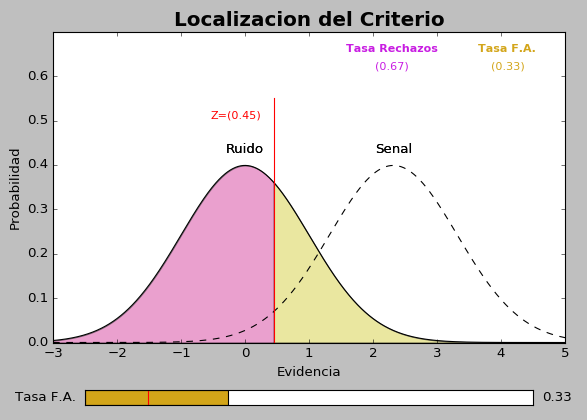
\includegraphics[width=0.90\textwidth]{Figures/Graficador_Criterio} 
%\decoRule
\caption[Estimación del criterio con base en las Falsas Alarmas]{Estimación de la localización del criterio sobre el eje de decisión con base en la tasa de Falsas Alarmas (y su complemento). La imagen presenta una captura de pantalla de un Graficador desarrollado por la autora de la presente tesis, como parte de un proyecto PAPIME trabajado en el Laboratorio 25, \parencite{PAPIME}}
\label{fig:Graf_Criterio}
\end{figure}

El parámetro $k$ representa la localización del criterio sobre el eje de decisión en unidades de \textit{desviación estándar}, \parencite{Tanner1954}. Su cómputo requiere interpretar la tasa de Falsas Alarmas como reflejo de la probabilidad acumulada -el área bajo la curva- de la distribución de Ruido que cae por encima del criterio, siendo su complemento la tasa de Rechazos Correctos. Dado que -de acuerdo con los supuestos formales previamente expuestos- se asume que la distribucion de Ruido tiene media en 0 y desviación estándar de 1, la tasa de Rechazos Correctos puede transformarse en \textit{Puntajes Z} para obtener un estimado -en términos del \textit{número de desviaciones estándar}- de dónde se sitúa el criterio de elección, tomando como referencia la media de la distribución de Ruido. La Figura~\ref{fig:Graf_Criterio} ilustra este proceso, presentando como ejemplo una tasa de Falsas Alarmas arbitraria y la tasa de Rechazos Correctos complementaria, que al ser transformada a puntajes Z permite evaluar la localización del criterio respecto del 0 de referencia planteado por la distribución de ruido. Es decir:\\

\begin{center}
$k = PuntajeZ(Tasa$ $de$ $Rechazos$ $Correctos)$\\
\end{center}

\item \underline{Discriminabilidad ($d'$)}\\

La discriminabilidad se evalúa con un parámetro $d'$ que define la distancia entre las medias de las distribuciones de Ruido y Señal, \parencite{Tanner1954}. Dado que a la distribución de Ruido le ha sido asignada una media en 0, también podemos pensar en $d'$ como la localización de la media de la distribución de Señal.\\ 

Una vez determinada la localización del criterio relativa a la media de la distribución de Ruido con base en las tasas de Falsas Alarmas y Rechazos Correctos observadas, es sencillo concebir el cómputo de $d'$ como una extensión de dicho procedimiento, utilizando las tasas de Hits y Omisiones para establecer la localización de la distribución de Señal sobre el eje de evidencia.\\ 

\begin{figure}[th]
\centering
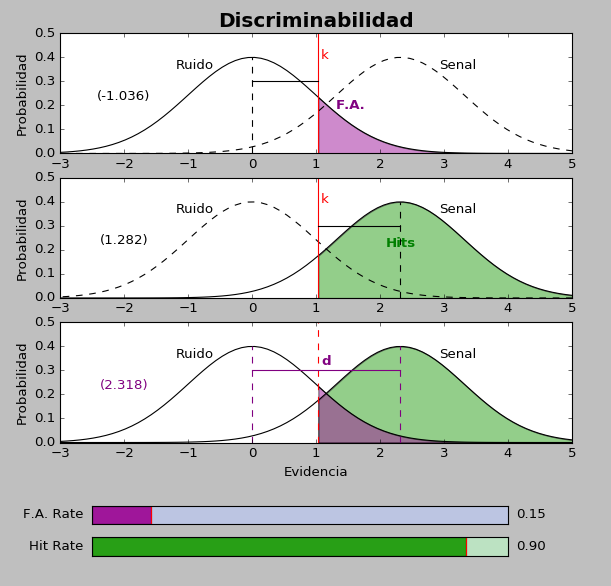
\includegraphics[width=0.80\textwidth]{Figures/Graficador_Discriminabilidad} 
%\decoRule
\caption[Estimación de la discriminabilidad con base en las Tasas de Ejecución]{Se ilustra la definición de la localización de la distribución de Señal en función a las tasas de Hits y Omisiones registradas, y la estimación subsecuente de la distancia entre las medias de ambas distribuciones. La imagen presenta una captura de pantalla de un Graficador desarrollado por la autora de la presente tesis, como parte de un proyecto PAPIME trabajado en el Laboratorio 25, \parencite{PAPIME}}
\label{fig:Graf_Discrim}
\end{figure}

La Figura~\ref{fig:Graf_Discrim} ilustra la secuencia lógica de pasos que guían el cómputo del valor de $d'$:\\

\begin{enumerate}
\item En el panel superior, la tasa de Falsas Alarmas (señalada en color púrpura) es convertida a Puntajes Z.\\

Pese a que conceptualmente interpretamos la tasa de Falsas Alarmas como la probabilidad acumulada por encima del criterio y esperaríamos un Puntaje Z positivo, el valor obtenido es negativo porque la conversión se hace bajo el entendido de que la probabilidad se acumula de izquierda a derecha (y no al revés, como implica nuestra interpretación). Es decir, el Puntaje Z obtenido para la tasa de Falsas Alarmas es negativo porque al ser menor a 0.5, se le asigna un Puntaje Z que obtendríamos si invirtiéramos la distribución y la probabilidad acumulada registrada se situara por debajo de la media.\\

El primer panel ilustra la estimación de la distancia entre el criterio y la media de la distribución Ruido.\\

\item El panel intermedio muestra el resultado de transformar la tasa de Hits (señalada en color verde) en puntajes Z.\\

A pesar de que la tasa de Hits señala que el criterio cae por debajo de la media de la distribución de Señal, el puntaje Z obtenido es positivo porque -nuevamente- la tasa de Hits registrada \textit{se lee} como una probabilidad acumulada de izquierda a derecha y dado que suele ser mayor al azar ($> 0.5$), representa un área bajo la curva que rebasaría la media de la distribución si esta estuviera invertida.\\

El segundo panel muestra el cómputo de la distancia entre el criterio y la media de la distribución Señal.\\

\item El panel inferior presenta lo que propiamente sería el cómputo de $d'$: la suma de las distancias entre el criterio y las medias de cada una de las distribuciones. Es decir:\\

\begin{center}
$d' = PuntajeZ(Tasa$ $de$ $Hits) - PuntajeZ(Tasa$ $de$ $Falsas Alarmas)$\\
\end{center}

\end{enumerate}

El parámetro $d’$ sólo puede tener valores positivos ya que la teoría asume que la distribución de Señal siempre se sitúa a la derecha de la distribución de Ruido, pues contiene más de la evidencia con base en la cual se hace el juicio de detección, \parencite{Stainslaw1999}.\\

El valor de $d'$ es un reflejo de la discriminabilidad en la tarea -la distancia entre las distribuciones-. Si $d' = 0$, querría decir que las distribuciones de Ruido y Señal están completamente sobrelapadas y es imposible distinguir entre ellas (\textit{'No hay discriminabilidad entre los estímulos'}). \\

\item \underline{Sesgo ($\beta$ y $C$)}\\

La SDT cuenta con dos parámetros que permiten evaluar la magnitud y la dirección del sesgo bajo el cual se está respondiendo a la tarea, \parencite{Stainslaw1999, Macmillan1996}.\\

\begin{itemize}
\item \underline{$\beta$}\\

El parámetro más comúnmente reportado en la literatura es Beta ($\beta$), que se define como la razón entre la densidad de probabilidad de la distribución Señal a la altura del criterio y la densidad de probabilidad  de la distribución Ruido: \\

\begin{center}
$\beta = \frac{p(Signal)}{p(Noise)}$ \\
\end{center}

En otras palabras, $\beta$ responde a la pregunta \textit{'¿Cuántas veces es más probable que la evidencia que corresponde con la localización del criterio sea una Señal y no Ruido?'}.

\item \underline{$C$}\\

Un segundo parámetro para computar el sesgo es $C$, que representa la distancia entre la localización del criterio utilizado por el sistema evaluado y el punto de intersección entre las distribuciones ($\frac{d'}{2}$):\\

\begin{center}
$C =  K - \frac{d'}{2}$ \\
\end{center}

Se utiliza $\frac{d'}{2}$ como punto de referencia para evaluar el sesgo del sistema porque se asume que esta debería ser la localización del criterio a utilizar por un sistema no sesgado, ya que el área de las distribuciones que cae por encima y por debajo de este punto son idénticas. En otras palabras, un criterio en $\frac{d'}{2}$ conllevaría a que exista la misma probabilidad de cometer ambos tipos de aciertos y errores. Por ello, el sesgo del sistema detector se evalúa a partir de su comparación con este punto neutro.\\

Es decir, el parámetro $C$ responde a la pregunta \textit{'¿Cuánto se aleja el criterio utilizado por el sistema de lo que se esperaría de un sistema sin sesgo?'}.\\

\end{itemize}

El sesgo puede ser evaluado en términos de dos factores: 1) ¿Qué tan sesgado está el sistema? y 2) ¿Cuál es el juicio de detección que se está favoreciendo?\\

El parámetro $\beta$ indica cuántas veces es más probable que la evidencia observada a la altura del criterio corresponda con la Señal. Valores de $\beta$ por encima de 1, sugieren que el punto en que la distribución de Señal toca el criterio es más alto que la distribución de Ruido; es decir, el sistema detector no emite juicios afirmativos hasta que exista una alta probabilidad de correspondencia entre la evidencia evaluada y la variabilidad contenida en la Señal y, por el contrario, emite juicios negativos con mayor probabilidad. Por su parte, valores de $\beta$ entre 0 y 1 sugieren que es más probable que la evidencia encontrada a la altura del criterio provengan de la distribución de Ruido; esto indicaría que el sistema detector está emitiendo juicios afirmativos aún cuando es más probable que la evidencia observada corresponda con el Ruido. Finalmente, cuando el criterio del sistema cae en el punto neutro previamente descrito ($\frac{d'}{2}$), $\beta$ vale 1, pues el criterio toca ambas distribuciones a la misma altura.\\

El valor absoluto del parámetro $C$ proporciona información sobre la magnitud del sesgo bajo el cual el agente detector evaluado está favoreciendo la emisión de cierto juicio sobre el otro. Adicionalmente, se puede saber la dirección en que se mueve el sesgo dependiendo de si $C$ tiene un valor positivo o negativo. Si $C$ es negativo, quiere decir que $k < \frac{d'}{2}$; es decir, que $k$ se sitúa a la izquierda del punto neutro y promueve por tanto una mayor cantidad de Hits y Falsas Alarmas al emitir más respuestas afirmativas. Si $C$ es positivo, quiere decir que $k > \frac{d'}{2}$ y se está promoviendo una tasa mayor de Rechazos Correctos y Omisiones.\\

En función de la dirección en que se presente el sesgo, el sistema evaluado puede clasificarse en una de tres categorías:\\

\begin{itemize}
\item \textsl{Sesgo liberal}. Se muestra una tendencia hacia la emisión de respuestas afirmativas (\textit{'Sí, la señal está presente'}) aún con niveles bajos de evidencia, pues el criterio se encuentra orientado a la izquierda del eje de evidencia. Es decir: \\
\begin{center}
$C < 0$\\
ó\\
$0 < \beta < 1$\\
\end{center}

\item \textsl{Sesgo conservador}. Se presenta una tendencia hacia la emisión de respuestas negativas (\textit{'No, la señal no está'}) pues el criterio se encuentra desplazado a la derecha del eje de evidencia, requiriendo una mayor cantidad de evidencia para la emisión de juicios afirmativos. Es decir: \\
\begin{center}
$C > 0$\\
ó\\
$\beta > 1$\\
\end{center}

\item \textsl{Sesgo neutro}. No se favorece ninguna de las dos respuestas y la probabilidad de cometer cualquier acierto o cualquier error es la misma; el criterio se encuentra en $\frac{d'}{2}$. Es decir: \\
\begin{center}
$C = 0$\\
ó\\
$\beta = 1$\\
\end{center}
\end{itemize}

En la Figura~\ref{fig:Graf_Sesgo} se muestra el cómputo de los dos parámetros de sesgo ($\beta$ en los paneles izquierdos y $C$ en los derechos), con ejemplos que ilustran un sesgo liberal (panel superior) con una alta probabilidad de cometer Hits y Falsas Alarmas y un sesgo conservador (panel inferior) donde los juicios de detección se emitidos sólamente al evaluar niveles altos de evidencia.\\

\begin{figure}[th]
\centering
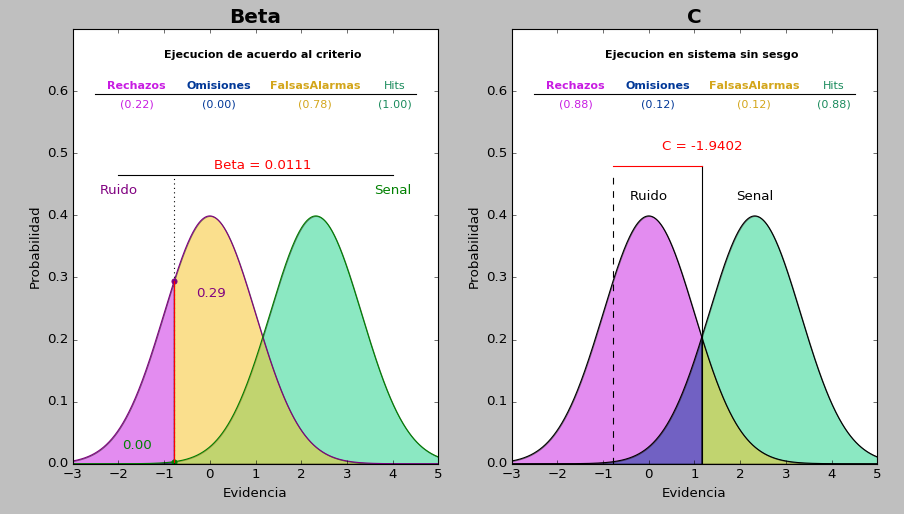
\includegraphics[width=0.65\textwidth]{Figures/Graficador_Sesgo_Liberal}\\
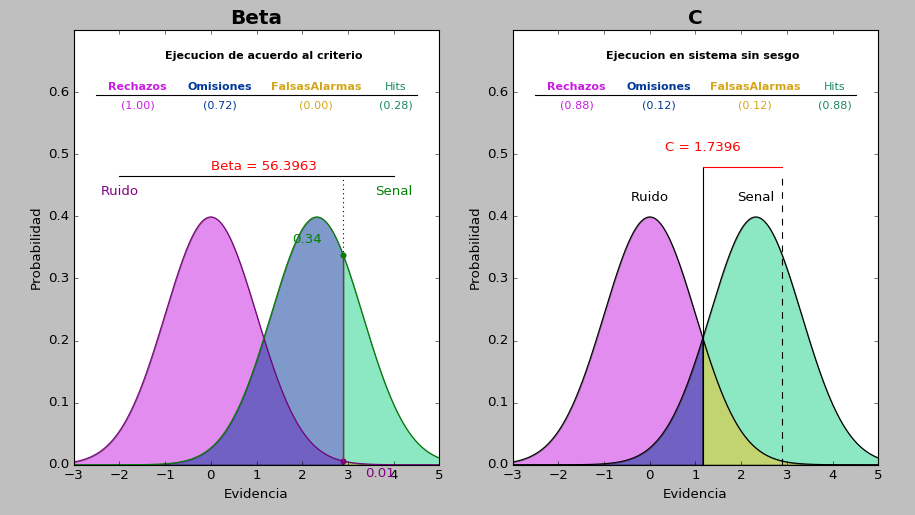
\includegraphics[width=0.65\textwidth]{Figures/Graficador_Sesgo_Conservador}\\
%\decoRule
\caption[Estimación del sesgo con base en el criterio]{Se ilustra el cómputo de los parámetros de sesgo $\beta$ (en los páneles izquierdos) y $C$ (en los páneles derechos), en casos donde el sesgo del sistema es liberal (panel superior) o conservador (panel inferior). La figura presenta capturas de pantalla de un Graficador desarrollado por la autora de la presente tesis, como parte de un proyecto PAPIME trabajado en el Laboratorio 25, \parencite{PAPIME}}
\label{fig:Graf_Sesgo}
\end{figure}
\end{itemize}   %Terminan los parametros

%----------------------------------------------------------------

\subsection{Curvas ROC}

Además de permitir la descripción e interpretación del desempeño observado en tareas de detección a partir de la estimación de los parámetros descritos, los datos obtenidos en sesiones experimentales pueden ser utilizados para una evaluación más completa de la precisión con que el sistema  podría responder a la misma tarea usando distintos criterio de elección. Las curvas ROC (identificadas así por su nombre en inglés: Receiver-Operating Characteristic curve) describen la relación entre la tasa en que las respuestas afirmativas emitidas son correctas o incorrectas -las tasas de Hits y Falsas Alarmas- en tareas de detección con cierto valor de $d'$, por cada localización posible del criterio sobre el eje de evidencia \parencite{McNicol2, Egan1959, Swets1973}.\\

La Figura~\ref{fig:Graf_ROC} ilustra la construcción de una curva ROC a partir de las tasas de ejecución reportadas en una tarea de detección. En el primer panel se presenta la representación gráfica del desempeño observado en un caso hipotético. En el panel intermedio se muestra la idea escencial del trazo de las curvas ROC, ubicando el punto de coordenadas que describe las tasas de Falsas Alarmas (en el eje de las x) y Hits (en el eje de las Y) representadas en el primer panel. Finalmente, para este mismo escenario (la misma $d'$), se presenta la curva ROC que representa los posibles intercambios entre las tasas de Hits y Falsas Alarmas que se espera obtener a traves del uso de los distintos valores posibles de $k$ sobre el eje de evidencia.\\

\begin{figure}[th]
\centering
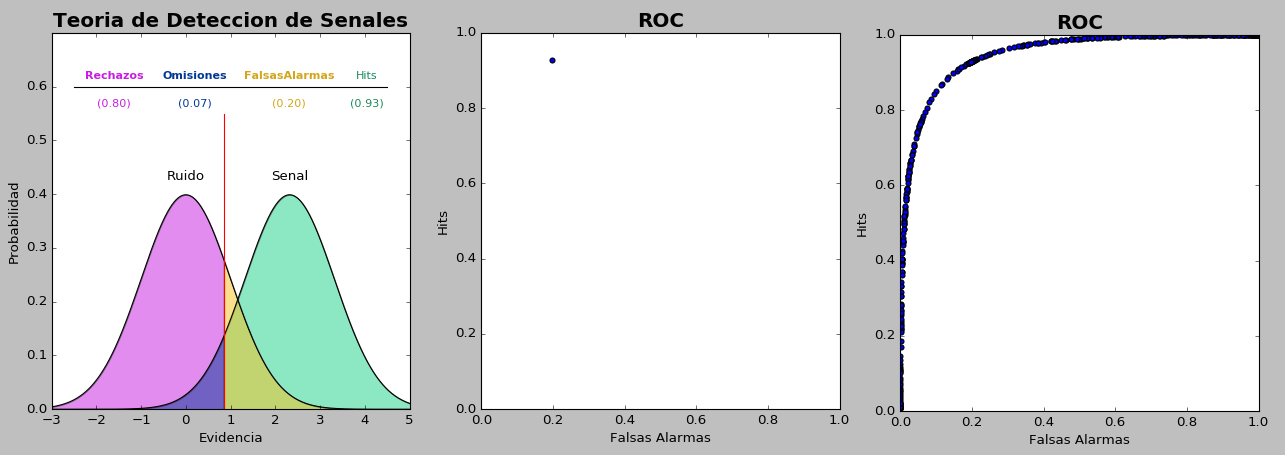
\includegraphics[width=0.90\textwidth]{Figures/Graficador_ROC12}\\
%\decoRule
\caption[Ejemplo de Curva ROC]{Se presenta la construcción de una curva ROC a partir del desempeño observado del sistema detector. El panel izquierdo presenta un ejemplo arbitrario con ciertas tasas de ejecución; el panel central traza con un solo punto las coordenadas que representan las tasas de hits y falsas alarmas observadas; y el panel derecho presenta la curva que se obtendría si trazáramos los puntos que representen las coordenadas correspondientes a cada localización posible del criterio. La figura presenta tres capturas de pantalla de un Graficador desarrollado por la autora de la presente tesis, como parte de un proyecto PAPIME trabajado en el Laboratorio 25, \parencite{PAPIME}}
\label{fig:Graf_ROC}
\end{figure}

Por cada valor de $d'$ se puede computar una sola curva ROC que describa los resultados esperados -en términos del intercambio entre Hits y Falsas Alarmas- para todas las posibles ubicaciones del criterio, \parencite{Tanner1954, Swets1961, Swets1973, Stainslaw1999}.\\

%Bajo el supuesto de que lo único sobre lo que el sistema detector tiene injerencia es sobre el criterio de elección a usar para emitir sus juicios de detección, y que la discriminabilidad -al ser una cualidad inherente a los estímulos comprometidos en la tarea (ya sea por la variabilidad en su presentación o percepción)- es constante y ajena a este, \\

El área bajo la curva ROC (AUC, por sus siglas en ingles: Area Under the Curve) representa una forma precisa y completa de evaluar la sensibilidad del sistema detector ante la tarea estudiada, \parencite{Centor1985,  Stainslaw1999, McNicol5}. Nótese que se habla de \textit{Sensibilidad} y no de \textit{Discriminabilidad} porque, aunque ambos conceptos refieren a qué tan fácil es para el sistema distinguir entre la Señal y el Ruido y están directamente relacionados con la distancia que existe entre sus distribuciones, la primera apela a la precisión con que el sistema detector puede responder a la tarea -utilizando distintas estrategias o reglas de elección- y la segunda hace referencia exclusivamente a una cualidad inherente a los estímulos, \parencite{Swets1973}.\\

El valor estimado de $d'$ representa la distancia entre las medias de las distribuciones y, como se mencionó anteriormente, en general se entiende que mientras más grande sea $d'$, más fácil es la tarea para el sistema involucrado en ella. Sin embargo, es complicado interpretar dicho valor en términos de qué tan \textit{buena} es la discriminabilidad; es decir, parece poco claro qué tanto tendría que alejarse el valor de $d'$ de $0$ para afirmar que la Señal es discriminable del Ruido. Para ello, el trazo de las curvas ROC y el cálculo del AUC correspondiente proporciona información valiosa para la evaluación de la precisión con que el sistema puede responder a la tarea de detección evaluada, si se usaran diferentes criterios, \parencite{Stainslaw1999}.\\ 

Cuando los estímulos con Señal son indistinguibles de los estímulos con Ruido ($d' = 0$), la curva ROC resultante se ve como una función de identidad. Esto implica que al emitir un juicio de detección afirmativo, existe la misma probabilidad de que este resulte en un Hit o una Falsa Alarma, con un AUC de 0.5 (la mitad del área total cae por debajo de la curva). Es decir, que mientras mayor sea el valor de $d'$, la curva ROC resultante se alejará más de la función identidad y su AUC será cada vez más cercano a 1.0. En general, el AUC puede tomar valores entre 0.5 -que correspondería a un sistema que no distingue en lo absoluto entre la Señal y el Ruido- y 1.0 -que representa una distinción perfecta entre los mismos-, \parencite{Swets1973, Stainslaw1999, McNicol5}.\\

Las curvas ROC pueden ser trazadas -en teoría- a partir de un solo conjunto de tasas de ejecución \parencite{Pollack1964a, Pollack1964b, McNicol2} mediante algoritmos que asumen que el desempeño observado por parte del participante no puede \textit{mejorar} o \textit{empeorar} (dado que la discriminabilidad no depende de su conducta) y que se limitan a computar las Tasa de ejecución que se esperaría observar en cada ubicación posible del criterio. Sin embargo, también pueden trazarse varios puntos para guiar el trazo de la curva ROC a partir de datos obtenidos en tareas de detección donde experimentalmente se induce el uso de distintos criterios de elección por parte de los participantes, obteniendo varios conjuntos de tasas de ejecucción (varias parejas de tasas de Hits y Falsas Alarmas), \parencite{Egan1959, Swets1961, Swets1986}. Los procedimientos mediante los cuales esto se lleva a cabo se discuten a continuación.\\

%----------------------------------------------------------------

\subsection{Tareas de detección}

En cuanto a la aplicación de la SDT a la interpretación y evaluación de la ejecución de cierto tipo de participantes en cierto tipo de tareas de detección, existen tres grandes protocolos empleados para presentar la tarea y obtener datos susceptibles de ser analizados bajo el marco del modelo propuesto, \parencite{McNicol2, Stainslaw1999}. A continuación se exponen de manera general las propiedades -en términos de la información que se obtiene- y especificaciones procedimentales que caracterizan a cada uno de ellos.\\

\begin{itemize}
\item \underline{Tareas de detección binaria}\\

La forma más sencilla y estándar de presentar una tarea de detección es con un procedimiento que únicamente solicite a los participantes la emisión de juicios binarios de detección (\textit{'Sí, la señal está'} o \textit{'No, no está'}). Dicho protocolo se identifica en la literatura con el nombre de \textbf{tareas de detección binaria} o \textbf{tareas Sí/No}, \parencite{McNicol2}.\\

Las tareas Sí/No realizadas en el laboratorio consisten en la presentación aleatoria de una serie de ensayos (N) compuesta por ensayos que contienen la señal (S) y ensayos con sólo ruido (R), siendo la única respuesta que los participantes deben registrar en cada ensayo, si la señal estuvo presente o no. Típicamente, la cantidad de ensayos S y R presentados durante la tarea es la misma. Esto es recomendable por dos grandes razones: 1) Garantiza que las tasas de Hits y Omisiones sean tan representativas del desempeño del participante a lo largo de la tarea experimental como las tasas de Falsas alarmas y Rechazos correctos, al darle el mismo número de oportunidades de cometer cada tipo de acierto y error, y 2) Evita que el sistema evaluado desarrolle un sesgo a favor de una respuesta particular en función a cuál es el tipo de ensayo que más se le presenta, \parencite{Nevin1969, Wickens}.\\

Por cada tarea Sí/No conducida, se obtiene un set de tasas de ejecución que permiten trazar uno solo de los puntos que componen la curva ROC que describiría la sensibilidad del sistema evaluado. Así que, para obtener más datos con los cuales trazar la curva (más puntos que representen un conjunto de tasas de ejecución), tendría que correrse la misma tarea en repetidas ocasiones, con los mismos estímulos y en los mismos participantes, pero incitando el uso de distintos criterios de elección en cada ocasión. Esto se puede hacer de manera explícita (solicitándole al participante que sea más o menos estricto en la emisión de sus respuestas), o implícita (presentando la tarea con diversas matrices de pago que promuevan que el participante evite un cierto tipo de error o busque aumentar cierto tipo de acierto), \parencite{Wickens, McNicol2}.\\

Un problema evidente con el trazo de curvas ROC a partir de los datos obtenidos en tareas de detección binarias repetidas es que se requiere un número considerable de repeticiones que deben estar compuestas por el mismo número de ensayos. Exponer a un mismo participante a la misma tarea y los mismos estímulos tantas veces trae consigo el riesgo de que su desempeño se vea afectado por la fatiga o el aprendizaje. Si este fuera el caso, los datos obtenidos no sólo serían reflejo de cambios en el criterio usado para responder a la tarea, sino que también podría haberse alterado la propia discriminabilidad de la tarea (el aprendizaje puede hacer que los participantes se vuelvan mejores distinguiendo entre la Señal y el Ruido, y la fatiga, tener el efecto opuesto). Esto representa un problema porque entonces, la curva ROC trazada no representaría la sensibilidad del sistema evaluado ante \textit{una misma} tarea, ya que se estaría violando el supuesto fundamental de que la discriminabilidad es constante, \parencite{McNicol2}.\\

\item \underline{Tareas con Escala de Confianza}\\

Una segundo protocolo para la presentación de tareas de detección -que puede ser entendida como una extensión del protocodo con tareas Sí/No- es solicitando a los participantes que respondan a la misma valorando y asignando un puntaje dentro de una \textbf{Escala de Confianza} que represente la certeza que tienen sobre la pertenencia de cada estímulo a las categorías Señal o Ruido.\\

En términos del procedimiento, las tareas de detección binarias y con Escala de Confianza son idénticas: se muestra a los participantes una serie de ensayos (N) dentro de la cual se presentan de manera aleatoria ensayos con la señal (S) y ensayos con sólo Ruido (R), solicitándoles que registren una respuesta al término de cada ensayo. La única diferencia entre ambos protocolos es el tipo de respuesta solicitada y, en consecuencia, la robustez de las estimaciones que pueden hacerse sobre la sensibilidad del sistema. En las tareas Sí/No los participantes emiten una de dos posibles respuestas mutuamente excluyentes; en tareas con Escala de Confianza, se asigna a cada estímulo evaluado un puntaje dentro de una Escala con cierto número de opciones de respuesta, \parencite{Stainslaw1999}.\\

Existen varias formas en que puede presentarse la Escala de Confianza, \parencite{McNicol2}. Por ejemplo, una de ellas podría ser solicitando que se responda de acuerdo a la confianza que se tendría en asignar cada estímulo evaluado a la categoria Señal (donde los valores más altos serían asignados a los estímulos que se encuentren más hacia la derecha en el eje de las evidencia y los valores bajos a los estímulos más a la izquierda, que podrían haber ser identificados como Ruido); una segunda forma, sería distinguiendo entre la certeza que se tiene sobre que el estímulo evaluado sea una Señal o Ruido, (los valores más altos reflejan la confianza que se tiene en que se trate de una Señal y los valores más bajos, a la certeza de que se trate de Ruido). Como se presenta en la tabla incluída en la parte superior de la Figura~\ref{fig:Conf_Rat}, ambas formas de presentar la Escala proporcionan -en teoría- la misma información y, en general, la elección de una u otra depende del experimentador.\\

El supuesto detras de la interpretación de los puntajes de confianza registrados, es que los participantes fijan un criterio sobre el eje de evidencia por cada opción de respuesta en la Escala de Confianza que va a determinar cuál de estos puntajes es emitido, dependiendo de cuál sea el último criterio de elección que la evidencia juzgada rebasa, \parencite{McNicol2}. La Figura~\ref{fig:Conf_Rat} ilustra esta idea: en la parte superior se presenta una Escala de Confianza de 6 elementos (se ejemplifican las dos formas -previamente expuestas- en que puede ser presentada), y en la parte inferior, la representación gráfica del modelo de detección de señales.\\

\begin{figure}[th]
\centering
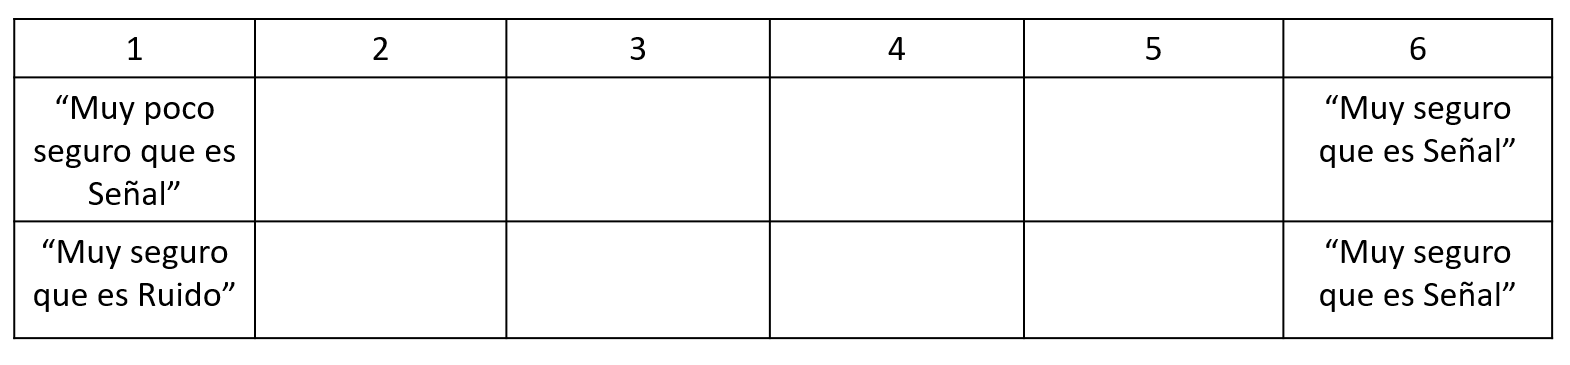
\includegraphics[width=0.80\textwidth]{Figures/Puntajes_Criterios}\\
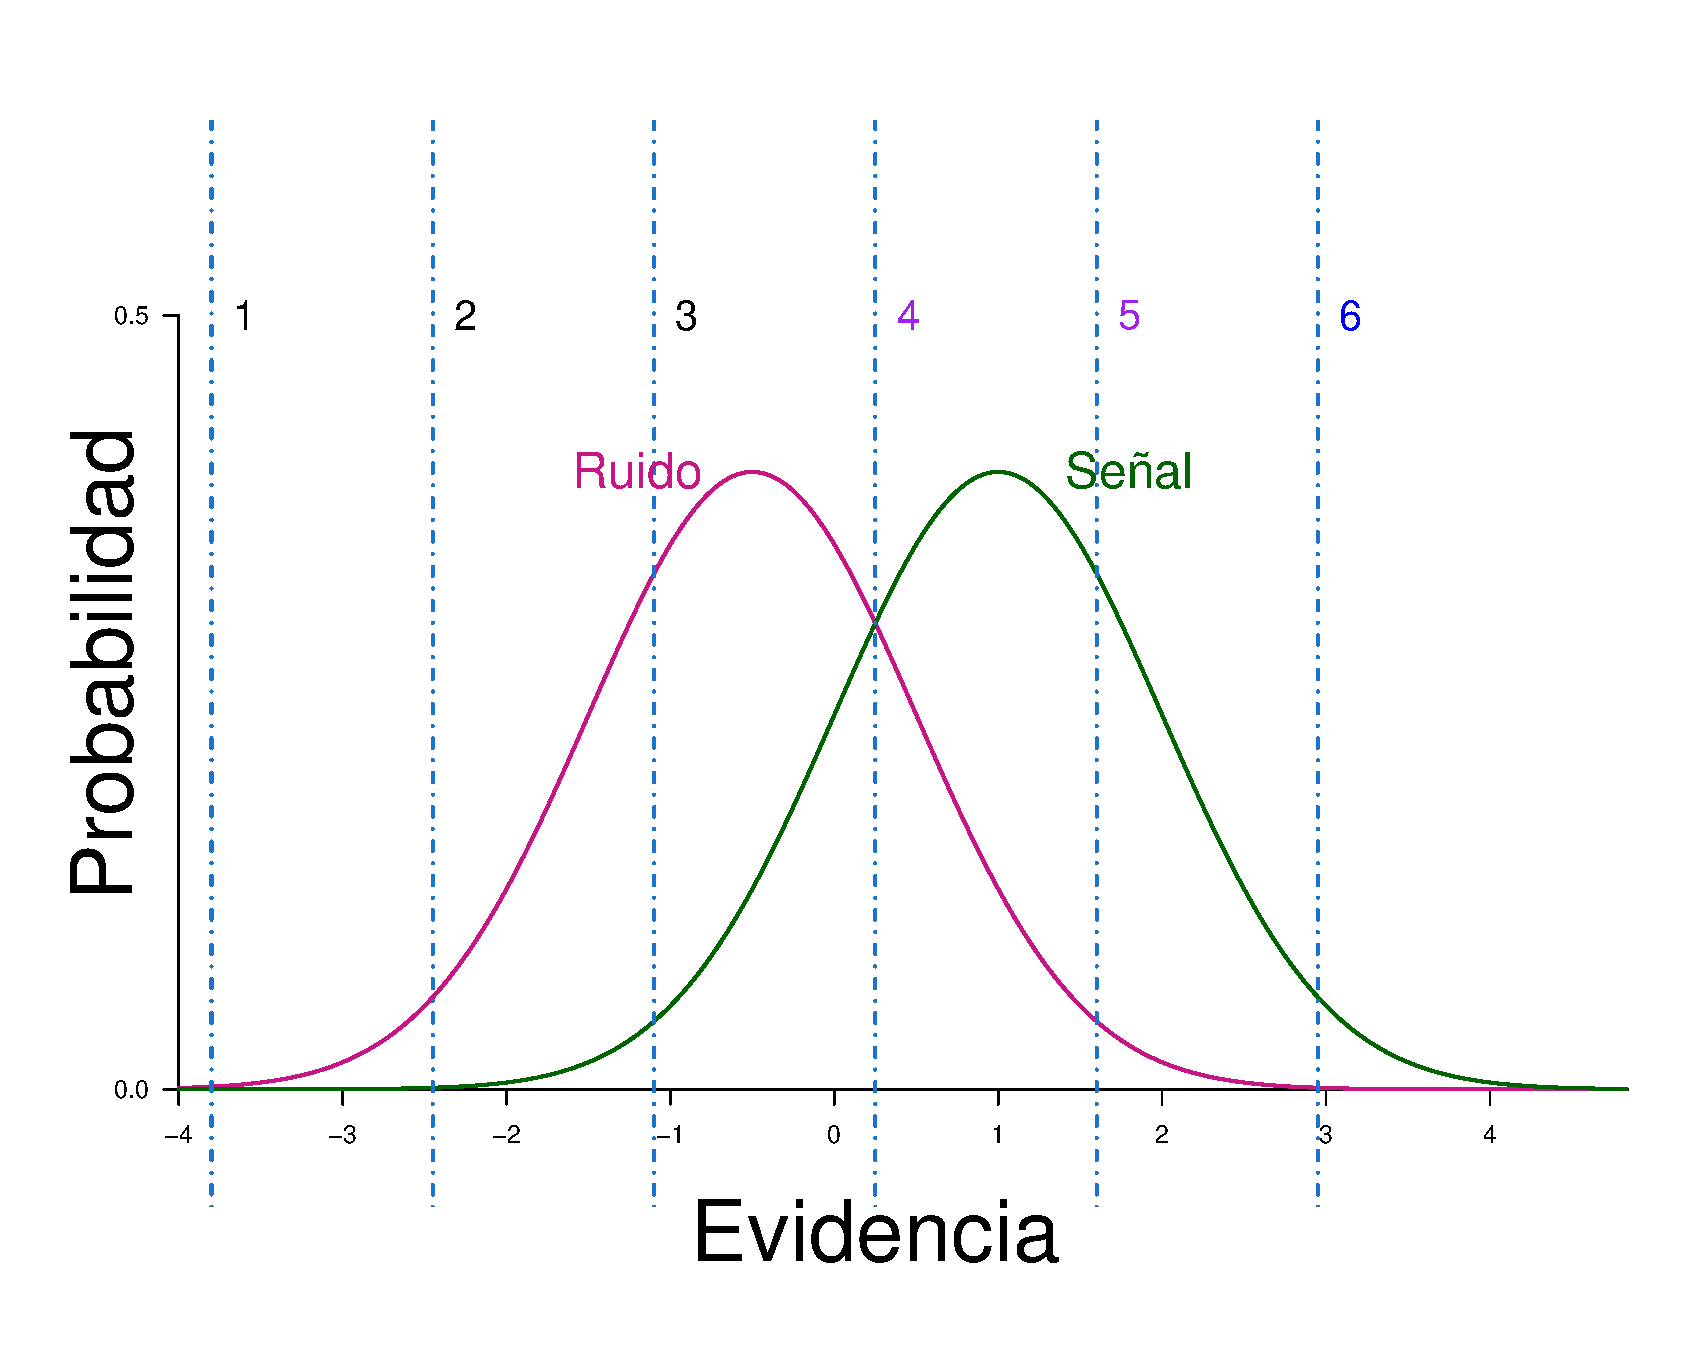
\includegraphics[width=0.70\textwidth]{Figures/ConfidenceRating}\\
%\decoRule
\caption[Representación gráfica de la interpretación de las tareas de detección con Escala de Confianza]{Representación gráfica de la interpretación de las tareas de detección con Escala de Confianza bajo el marco de la SDT. En la parte superior se presenta una Escala de Confianza de seis elementos con sus dos posibles direcciones: unidireccional (el puntaje refleja la confianza en una sola respuesta) o bidireccional (el puntaje distingue entre la confianza en cada respuesta). La gráfica de abajo ilustra la idea de que por cada puntaje se computa la localización de un sub-criterio sobre el eje de evidencia, a partir del número de Hits y Falsas Alarmas que se obtendrían de haber utilizado dicho puntaje como una respuesta afirmativa en una tarea binaria.}
\label{fig:Conf_Rat}
\end{figure}

El protocolo de Escala de Confianza permite -en un mismo experimento- recoger datos que representen el uso de criterios múltiples -tantos como opciones de respuesta se incluyan en la Escala- por parte del sistema detector en una misma tarea de detección, permitiendo asumir que la discriminabilidad se mantiene constante. Por ello, el uso de Escala de Confianzas con $n$ opciones de respuesta, representa una forma sencilla y directa de obtener datos suficientes para trazar puntos ($n - 1$) que permitan trazar la curva ROC que represente la sensibilidad del sistema, \parencite{Stainslaw1999, McNicol2, McNicol5}.\\ 

Idealmente, se espera que el participante utilice todas las opciones de respuesta incluídas en la Escala de Confianza. Esto se puede conseguir de manera explícita o implícita, solicitando a los participantes que lo hagan así, o bien, modificando el número de puntajes incluídos en la Escala. En general, se recomienda que la Escala esté compuesta por un número par de opciones de respuestas que oscile entre 4 y 10 \parencite{McNicol2, McNicol5}. Esto con el fin de evitar que los participantes elijan la opción intermedia siempre que se sientan inseguros sobre su respuesta.\\

\item \underline{Tarea de Elección forzada}\\

Existe un tercer protocolo bajo el cual se presentan las tareas de detección, identificado como \textbf{tareas de Elección forzada entre $m$ alternativas}, donde se presentan simultáneamente $m - 1$ estímulos que contienen sólo ruido y $1$ con señal, y la tarea del participante consiste en identificar la Señal dentro del conjunto de estímulos que se le presentan, \parencite{Stainslaw1999}. En general, se asume que cada estímulo presentado contiene cierto valor de evidencia -cierta ubicación en el eje sobre el cual se despliegan las distribuciones- que el participante compara para elegir aquel que tenga un valor mayor -de acuerdo con el supuesto que establece que, en general, los valores de la distribución Señal caen por encima del Ruido-, \parencite{McNicol2}.\\

Dada la relación que representan, el área bajo la curva ROC trazada con un protocolo de preguntas binarias o con Escala de Confianza puede interpretarse como la proporción de veces que el participante cuyo desempeño se describe, podría identificar correctamente la Señal, si esta fuera presentada simultáneamente junto con el Ruido. A su vez, la proporción de respuestas correctas obtenidas a lo largo de una tarea de Elección forzada proporciona una medida de la sensibilidad del sistema, independiente del sesgo del sistema. Dicha medida -al igual que el AUC-, tendría que variar entre el azar ($\frac{1}{m}$) y el desempeño perfecto ($1.0$), \parencite{Stainslaw1999}.\\
\end{itemize}


















\section{Teoría de Detección de Señales en Memoria}

La Teoría de Detección de Señales ha sido ampliamente utilizada en distintas áreas de la Psicología Experimental tanto como marco de referencia conceptual para la descripción de diversas situaciones de detección, como herramienta para el análisis de datos obtenidos en dichas tareas. Una de estas áreas refiere al estudio de la Memoria, donde los supuestos y conceptos desarrollados en la SDT han sido aplicados para explicar el funcionamiento del aprendizaje humano, la retención, el olvido y el reconocimiento de estímulos, \parencite{Murdock1965, Bernbach1967, Lockhart1970, Banks1970, White1999}.\\

Al diseñar las tareas presentadas en estudios de Memoria como instancias de un problema de detección, los resultados obtenidos pueden clasificarse dentro de las mismas categorías que en cualquier procedimiento estándar de detección de señales (identificadas en cada una de las celdas que componen la matriz presentada en la Figura~\ref{fig:Mat_Output}), en función de la correspondencia entre la respuesta registrada por los participantes y el tipo de ensayo evaluado. Y a su vez, las tasas de Hits y Falsas Alarmas registradas por cada criterio evaluado (en tareas Sí/No que inducen distintos sesgos o mediante el uso de Escalas de Confianza) permiten el trazo de curvas ROC \parencite{Egan1958, VanZ2000}, con frecuencia identificadas como curvas MOC (por sus siglas en inglés \textit{Memory Operant Curve}) para enfatizar su adscripción al estudio de la Memoria, \parencite{Norman1965, KintschCarlson1967}.\\

La aplicación de la SDT al estudio de la Memoria ha impactado en el desarrollo de este útlimo en términos de cuatro grandes ejes \parencite{Banks1970}, que son:\\

\begin{enumerate}
\item La noción de la \textit{Fuerza de Memoria}.\\

Aceptar la SDT como marco para describir el funcionamiento de los distintos mecanismos estudiados en Memoria y el desempeño observado en participantes sometidos a distintas tareas, implica asumir que el \textit{input} con base en el cual se emiten las respuestas ensayo a ensayo son valores ($x$), que representan distintos puntos dentro del eje de evidencia sobre el cual se despliegan las distribuciones de Ruido (los estímulos distractores) y Señal (los estímulos a identificar de acuerdo al procedimiento empleado). Típicamente, se entiende dicho valor $x$ como un reflejo de la \textit{fuerza de memoria}, o bien, un índice de qué tan \textit{relacionable} o \textit{familiar} resulta para el sistema cada estímulo evaluado, \parencite{Ratcliff1992}. Así pues, los modelos de memoria que incorporan la SDT como base para el desarrollo de su marco explicativo interpretan el desempeño observado en los participantes como resultado de la interacción entre la \textit{fuerza de memoria} evaluada en cada ensayo y un proceso de decisión que determina si ésta es lo suficientemente grande para juzgar la pertenencia de cada estímulo a la categoría Señal.\\

En términos de la exploración de este supuesto y sus implicaciones, resaltan los trabajos orientados a evaluar la naturaleza de dicha \textit{fuerza de memoria} (por ejemplo, si puede entenderse a partir de valores contínuos o discretos), y su interacción con los procesos propios de la Memoria (por ejemplo, el estudio, la retención y el olvido), \parencite{Bernbach1967, Wickelgren1966, Parks1966}.\\

\item La noción del Criterio de Elección como opuesta a los Umbrales de respuesta.\\

Una de las aportaciones más evidentes de la aplicación de los principios propuestos por la SDT al estudio de la Memoria es que permite entender los Falsos Positivos en términos de una confusión entre la fuerza de memoria producida por un estímulo distractor y la Señal (el área de sobrelape entre las distribuciones), y abandonar el supuesto de que cuando las señales a detectar están ausentes, los participantes responden a la tarea de manera aleatoria. En otras palabras, se abandona la noción originada en torno a la Teoría del Umbral de que existe tal cosa como un \textit{umbral de memoria} que debe ser rebasado para que el sistema sea capaz de identificar la pertenencia de los estímulos a una u otra categoria, \parencite{Murdock1982, Gillund1984, Yonelinas1996, Wixted2007}. Con ello, tal y como ocurrió tras la incorporación de la SDT al estudio de la Percepción, se admite la conceptualización de los procesos de Memoria como instancias de un proceso de decisión \parencite{Bernbach1967}.\\
 
\item La noción de que existen distribuciones subyacentes (y la definición de sus características).\\

Como se mencionó previamente, los datos obtenidos en experimentos de memoria donde se promueva el uso de diversos criterios de elección pueden utilizarse para construir curvas MOC que describan la precisión con que los participantes distinguen entre los estímulos ruido y señal. A su vez, dado que cada curva representa un solo valor de $d'$, que se asume permanece constante a lo largo del uso de distintos criterios de elección, las curvas MOC permiten evaluar qué tipo de distribuciones permiten explicar mejor la relación registrada entre las tasas de Hits y Falsas Alarmas, \parencite{Kintsch1967, Ratcliff1992, Ratcliff1994}. Específicamente, cuando las curvas MOC son trazadas en términos de los puntajes Z que corresponden a las tasas de Hits y Falsas Alarmas como indicadores de la densidad de probabilidad acumulada en los extremos superiores las distribuciones de Señal y Ruido, respectivamente, se obtienen las llamadas curvas z-ROC que arrojan información sobre la naturaleza de las distribuciones subyacentes, \parencite{Ratcliff1992}, en términos de tres grandes factores:\\

\begin{itemize}
\item Si la curva z-ROC trazada es una línea recta, se acepta el supuesto de que las distribuciones de Ruido y Señal subyacentes son normales.\\
\item La pendiente de la curva z-ROC permite conocer la razón entre las desviaciones estándar de las distribuciones de Ruido y Señal.\\
\item El intercepto de la curva z-ROC proporciona información sobre la distancia entre las distribuciones ($d'$).\\
\end{itemize}

\item Análisis de datos y descripción del desempeño de los participantes.\\

Finalmente, se encuentran los trabajos que se limitan a utilizar la SDT como herramienta para analizar e interpretar los datos obtenidos en estudios de memoria que incorporan la metodología asociada con tareas de detección, \parencite{Marks1964, Wickelgren1966_Solo, Schulman1967}.\\
\end{enumerate} 

\subsection{ Memoria de Reconocimiento}

Por mucho tiempo, los modelos desarrollados en Memoria estuvieron muy limitados en términos del espectro de tareas y fenómenos de los que permitían dar cuenta \REFERENCIAS. No fue hasta que comenzaron a surgir los \textit{modelos globales de memoria} que incorporaron los principios básicos de la SDT para dar cuenta del funcionamiento de la Memoria humana, que fue posible explicar una gama más amplia de tareas y mecanismos comprendidos dentro del área con un mismo modelo. Estos modelos se distinguen principalmente por el tipo de supuestos que proponen acerca del tipo de distribuciones que podrían describir la variabilidad contenida en los estímulos con ruido y señal, o bien, sobre la forma en que se define la fuerza de memoria a partir de la interacción entre los distintos sistemas de memoria y los estímulos, \parencite{Murdock1982, Gillund1984, Eich1985}. Cada uno de estos modelos ha sido desarrollado para dar cuenta de un sub-set específico de tareas y fenómenos (recuerdo, juicios de frecuencia, olvido y retención, entre otros) y convergen en el estudio de la Memoria de Reconocimiento, \parencite{Parks1966, Ratcliff1992}.\\

Los modelos que incorporan la SDT para dar cuenta de la Memoria de Reconocimiento aparecen como una alternativa a los modelos clásicos que adoptaban la idea de \textit{umbrales de respuesta}. Un ejemplo representativo de este tipo de aproximación es la Teoría del Procesamiento Dual que plantea que existen dos procesos fundamentales involucrados en la emisión de los juicios de reconocimiento (la recolección y el análisis de familiaridad), que van a \textit{tomar control} de la tarea en función a qué tan familiar sea el estímulo evaluado \parencite{Yonelinas1996, Wixted2007}.

Aplicar la SDT al estudio de la Memoria de Reconocimiento implica entender las tareas de reconocimiento como una instancia de tareas de detección, donde los participantes tienen que identificar cuáles de los elementos que se le presentan dentro de una lista ya se le habían mostrado con anterioridad en una fase previa de estudio (los \textit{estímulos viejos}: las señales) y cuáles no (los \textit{estímulos nuevos}: el ruido), \parencite{Bernbach1967, Kintsch1967}. Se asume también que la 'fuerza de memoria' refleja el grado en que un estímulo cualquiera es percibido como 'familiar' para el sistema y que es el resultado de su comparación con un criterio de elección lo que determina la respuesta a registrar (\textit{'Sí, es un elemento antes visto'} o \textit{'No'}).\\ 

\begin{figure}[th]
\centering
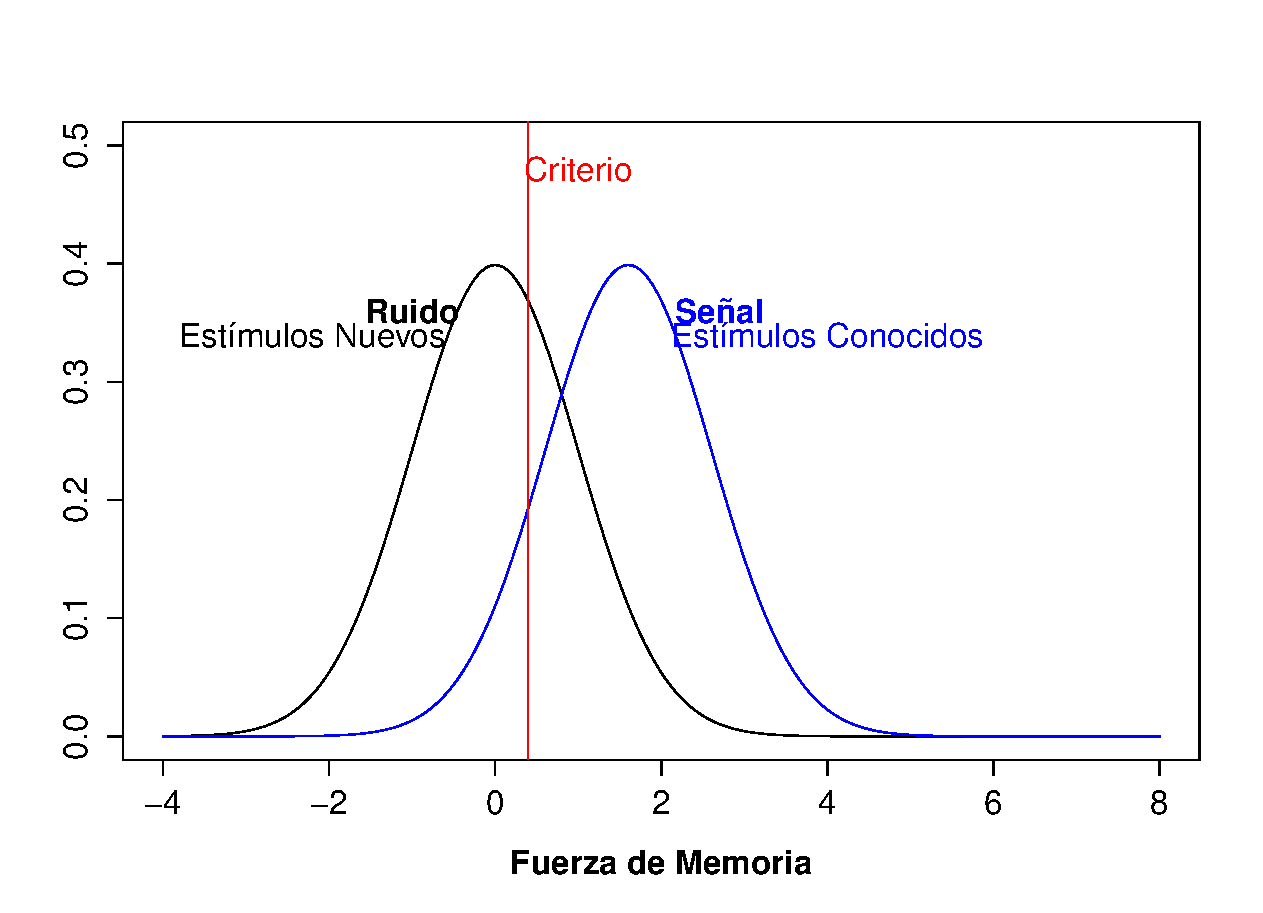
\includegraphics[width=0.60\textwidth]{Figures/RM_SDT_1} 
\decoRule
\caption[SDT en Memoria de Reconocimiento]{Modelo de Detección de Señales aplicado al estudio de Memoria de Reconocimiento}
\label{fig:RM_SDT_1}
\end{figure}

La Figura~\ref{fig:RM_SDT_1} ilustra la forma en que los supuestos y conceptos básicos de la SDT se aplican al contexto de la Memoria de Reconocimiento. La Señal representa los estímulos ya conocidos (típicamente referidos como \textit{estímulos viejos}) y el Ruido se compone por estímulos nuevos que pueden -o no- ser confundidos con los primeros. El \textit{eje de evidencia} a lo largo del cual se despliegan las distribuciones de Ruido y Señal, se convierte en un \textit{eje de familiaridad} que contiene distintos valores de 'fuerza de memoria' (y al igual que en la SDT clásica, se espera que los estímulos pertenecientes a la distribución Señal tengan valores más altos de 'familiaridad' que aquellos nunca antes vistos). Por último, se incorpora la idea de que la emisión de juicios de reconocimiento depende del contraste entre la 'familiaridad' evaluada en cada ensayo y un criterio de elección.\\

Las tareas de reconocimiento conducidas en el laboratorio suelen componerse de dos fases, \parencite{Ratcliff1992}. En la primera (\textit{la fase de estudio}) se presenta a los participantes una serie de elementos para que los estudien de manera intencional (solcitándoles explícitamente que las estudien para su reconocimiento posterior) o incidental (planteándoles alguna tarea distractora que los obligue a interactuar con ellos), \parencite{Noldy1990}. En la segunda fase (la \textit{fase experimental} o \textit{de reconocimiento}) se presentan los mismos elementos incluidos en la primera, más una cantidad igual de elementos nunca antes presentados, y se asigna a los participantes la tarea de identificar cuáles de los elementos incluidos en esta segunda fase son \textit{viejos} o \textit{nuevos}.\\

De acuerdo a las características de las curvas z-ROC construidas consistentemente a partir de datos empíricos en tareas de reconocimiento, parece ser que los modelos de memoria basados en la SDT que mejor predicen y se ajustan al desempeño observado en participantes de este tipo de tareas, son aquellos que asumen que las distribuciones subyacentes de Ruido y Señal son normales. Más aún, dada la pendiente que suele reportarse en este tipo de curvas, parece ser que la distribución de Ruido tiene una varianza menor a la distribución de Señal, \parencite{ Ratcliff1992, Ratcliff1994}. Tal y como se ilustra en la Figura~\ref{fig:RM_SDT_2}, consistentemente la razón entre la desviación estándar de la distribución de Ruido y la desviación estándar de la Señal tiene un valor al rededor de 0.8, \parencite{Wixted2007}.\\

\begin{figure}[th]
\centering
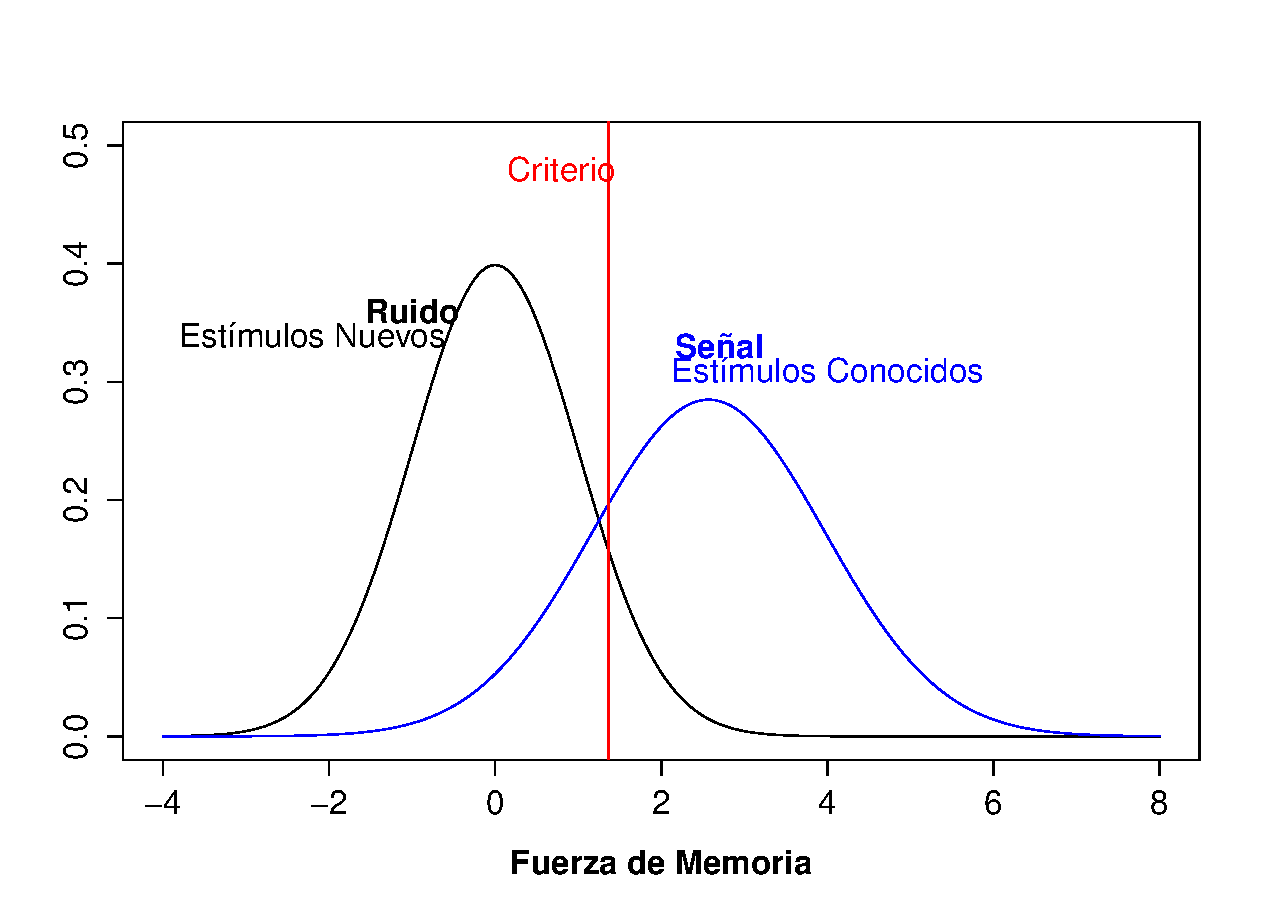
\includegraphics[width=0.60\textwidth]{Figures/RM_SDT_2} 
\decoRule
\caption[SDT en Memoria de Reconocimiento (Varianzas Desiguales)]{Modelo de Detección de Señales con varianzas desiguales aplicado al estudio de Memoria de Reconocimiento}
\label{fig:RM_SDT_2}
\end{figure}














\section{El Efecto Espejo}

El 'Efecto Espejo' refiere a un patrón de respuestas reportado consistentemente en estudios de Memoria de Reconocimiento analizados bajo el marco de la SDT, donde se compara el desempeño de los participantes entre dos clases de estímulos que difieren en la precisión con que suelen reconocerse tras presentarse una vez. Típicamente, dichas clases son referidas en la literatura como Clase A, con estímulos fácilmente reconocibles, y Clase B, con estímulos que se reconocen con mayor dificultad, (siendo que $d'(A) > d'(B)$), \parencite{Glanzer1990}. En dichos experimentos se ha encontrado evidencia sólida de que la diferencia entre la discriminabilidad con que se distinguen los elementos Nuevos y Viejos de las clases A y B se manifiesta en dos sentidos: en la identificacíón de los estímulos viejos como \textit{Viejos} (más Hits en A que en B) y en la identificación de los estímulos nuevos como \textit{Nuevos} (menos Falsas Alarmas en A que en B). Es decir, las diferencias en $d'$ parecen repercutir no sólamente en la cantidad de aciertos cometidos, sino también en los errores, \parencite{Glanzer1993}.\\

Al interpretar bajo el marco de la SDT las diferencias entre la proporción de Hits y Falsas Alarmas reportadas en las clases A y B, se sugiere que existen cuatro distribuciones subyacentes a la presentación de los estímulos Viejos y Nuevos de las clases A y B, siendo que el orden en que se presentan las distribuciones de estímulos Viejos A y B es el reflejo (\textit{mirror}) del orden en que se presentan las distribuciones de estímulos Nuevos de cada clase, \parencite{Glanzer1990, DeCarlo2007}. La representación gráfica de este orden (Nuevos(A), Nuevos(B), Viejos(B) y Viejos(A)), se presenta en la Figura~\ref{fig:Ejem_EfectoEspejo} y constituye la razón principal por la cual se ha identificado dicho patrón de respuesta con el nombre de Efecto Espejo.\\

\begin{figure}[th]
\centering
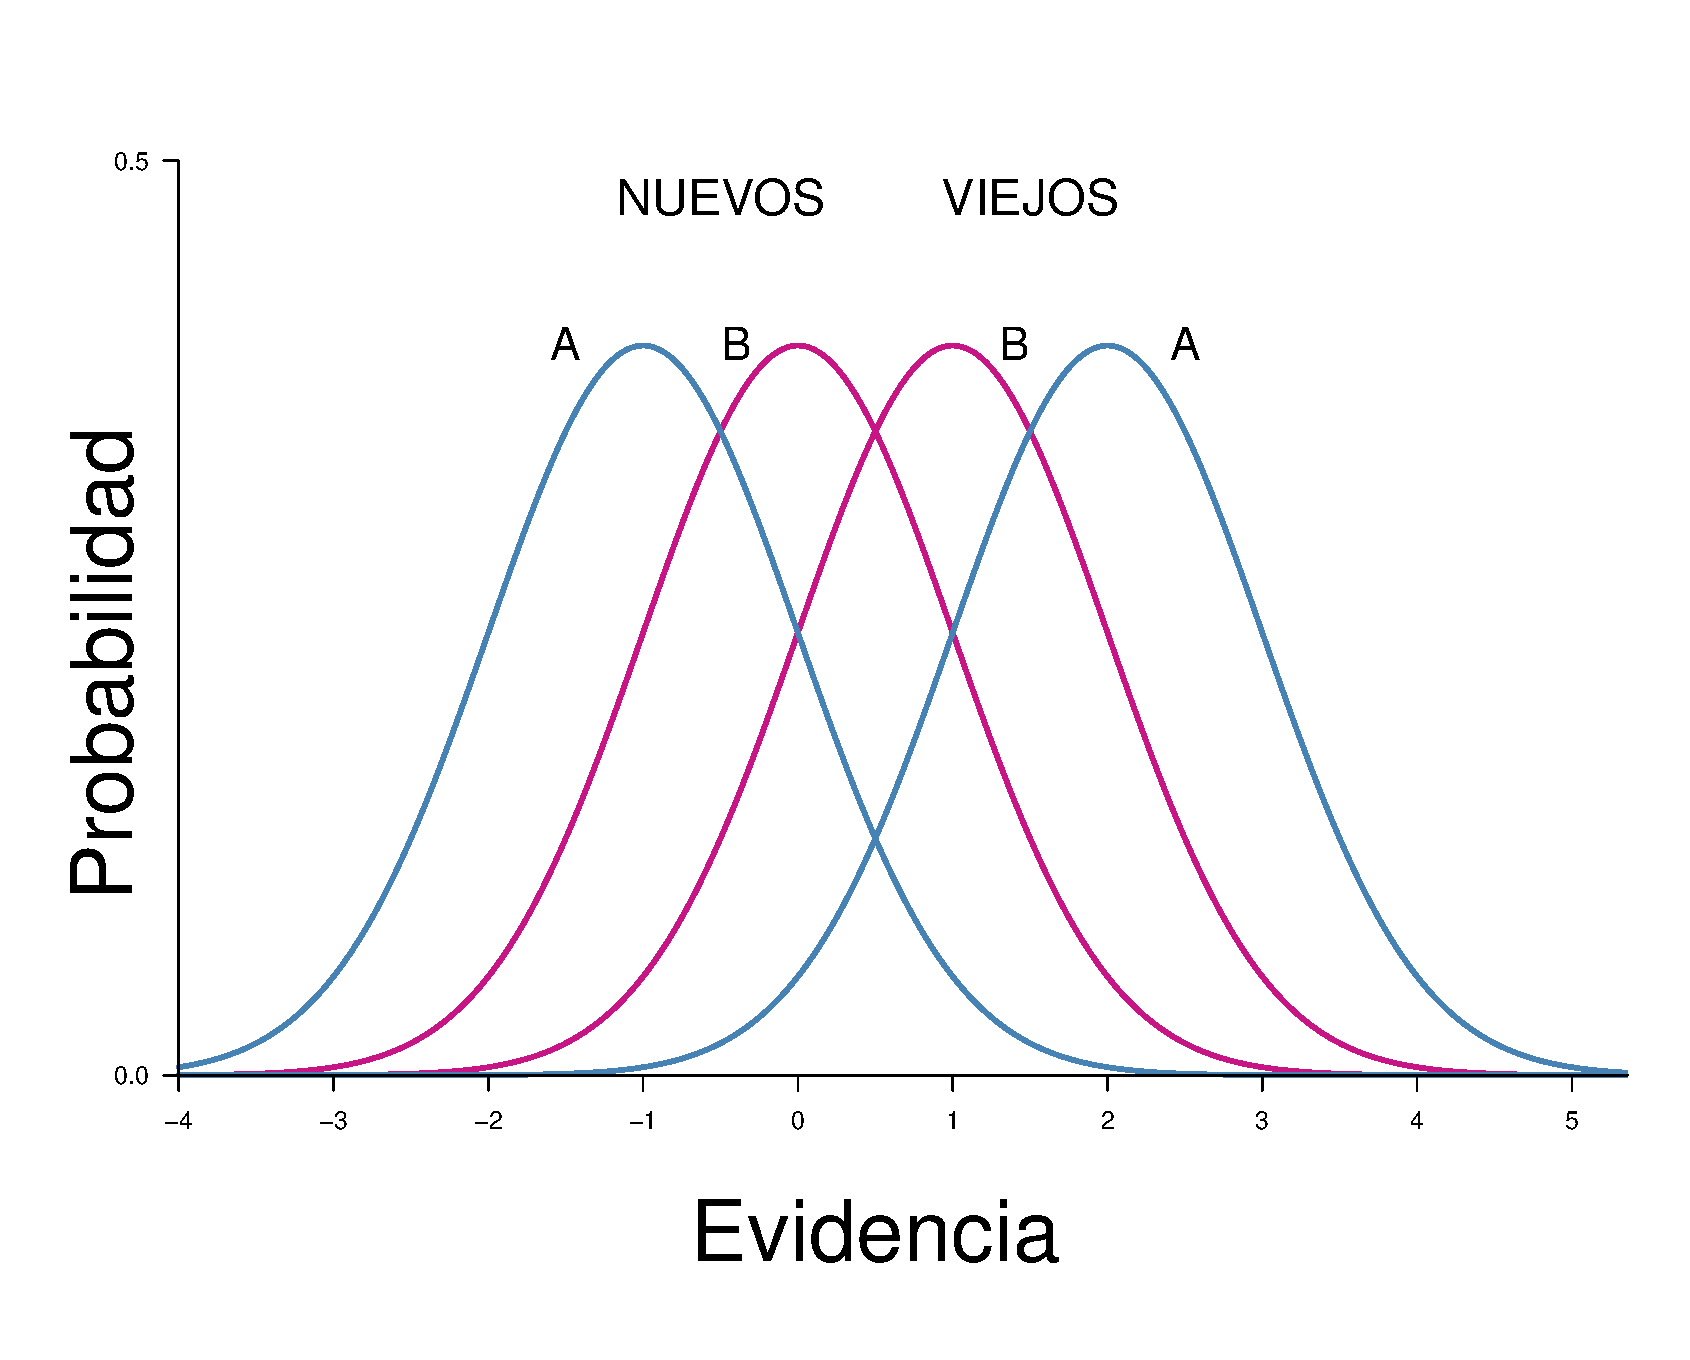
\includegraphics[width=0.7\textwidth]{Figures/EfectoEspejo}
%\decoRule
\caption[Representación gráfica del Efecto Espejo]{}
\label{fig:Ejem_EfectoEspejo}
\end{figure}

La evidencia a favor del Efecto Espejo en experimentos de Memoria de Reconocimiento se reporta a lo largo de una amplia variedad de tipos de \textit{clases de estímulos} y protocolos de tareas de detección (Preguntas Sí/No; Escala de Confianza y Elección Forzada de dos alternativas), \parencite{Glanzer1990}, que comparten las siguientes condiciones:\\

\begin{itemize}
\item Existen al menos dos clases de estímulos -típicamente identificados con las letras A y B- entre los cuales se compara el desempeño de los participantes, que difieren en su nivel de discriminabilidad: una clase de estímulos (A) se caracteriza porque se reconocen con mayor facilidad que los estímulos contenidos en la segunda clase (B) al ser presentados en más de una ocasión.\\

\item Los estímulos que componen las clases A y B se presentan de manera simultánea y aleatoria durante la tarea, tanto en la fase de estudio como en la fase de reconocimiento, sin que los participantes tengan forma de saber que se le está presentando más de un tipo de estímulo o  que su desempeño se va a evaluar en términos de las diferencia con que respondan a cada uno de estos. Esto se procura por dos razones: 1) permite asumir que el participante está respondiendo con base en un sólo criterio de elección y 2) permite controlar la forma en que las distribuciones subyacentes se escalan, \parencite{DeCarlo2007}.\\
\end{itemize}

La separación que se observa en la Figura~\ref{fig:Ejem_EfectoEspejo} entre las distribuciones de estímulos Viejos A y B tiene sentido bajo el supuesto de que las tareas de reconocimiento funcionan como una instancia de detección de señales, ya que se espera que exista una mayor distancia entre la distribución Señal asociada con una $d'$ más grande (Viejos(A)) y el Ruido. Sin embargo, no habría razón para esperar que dicha diferencia se repita y \textit{refleje} entre las distribuciones de estímulos Nuevos A y B, pues en el contexto del estudio de la Memoria de Reconocimiento no hay cómo explicar que el desempeño de los participantes difiera entre los estímulos Nuevos A y B (el ruido) bajo el supuesto de que se trata de estímulos que no han sido mostrado previamente. En otras palabras, no hay forma de justificar las discrepancias reportadas en el Efecto Espejo entre las Falsas Alarmas en A y B, puesto que la \textit{familiaridad} de sus estímulos debería ser igual según los modelos de memoria desarrollados hasta el momento, \parencite{Glanzer1993}.\\

\subsection{Evidencia recolectada}

Como se mencionó previamente, la evidencia del Efecto Espejo en tareas de Memoria de Reconocimiento analizadas bajo el marco de la SDT se presenta de manera consistente a lo largo de distintos protocolos experimentales, \parencite{Glanzer1990, Glanzer1993}. Los patrones de respuesta identificados en cada caso y su relación con el Efecto Espejo y su representación gráfica (presentada en la Figura~\ref{fig:Ejem_EfectoEspejo}), se exponen en detalle a continuación:\\

\begin{itemize}
\item \underline{Efecto Espejo en Tareas Sí/No}\\

En el caso de las tareas Sí/No, donde durante la fase de reconocimiento se presenta a los participantes aleatoriamente estímulos Nuevos y Viejos de las clases A y B para que emitan una respuesta Sí/No, con la cual señalen si les reconocen como parte de la fase de estudio (la Señal: \textit{'Sí, es un estímulo Viejo'}), o no (el Ruido: \textit{'No, es un estímulos Nuevo'}), se reporta el siguiente patrón de respuestas:\\

\begin{center}
$p[Si(NuevoA)] < p[Si(NuevoB)] < p[Si(ViejoB)] < p[Si(ViejoA)]$\\
\end{center}
\begin{center}
donde $p[Si]$ es la proporción de juicios de reconocimiento afirmativos emitidos (\textit{'Sí, este estímulo se me había presentado antes'}), $A y B$ son las clases de estímulos a comparar y $Nuevo y Viejo$, la pertenencia de los estímulos presentados a las categorías Ruido o Señal, \parencite{Glanzer1993}.\\
\end{center}

De acuerdo con la correspondencia entre el tipo de estímulo presentado y los juicios de reconocimiento afirmativos emitidos, esta misma relación puede definirse en términos de Hits y Falsas Alarmas, de la siguiente manera:\\

\begin{center}
$FA(A) < FA(B) < H(B) < H(A)$\\
\end{center}
\begin{center}
donde $FA$ y $H$ señalan las tasas de Hits y Falsas Alarmas observadas durante la tarea en cada clase, \parencite{Glanzer1993}.\\
\end{center}

De acuerdo con la interpretación clásica de este tipo de tareas en el marco de la SDT, se asume que los participantes emiten sus juicios de reconocimiento a partir de un criterio de elección y su comparación con la evidencia evaluada ensayo a ensayo -un valor $x$ que representa una posición específca sobre el eje de evidencia-, con lo que determina si esta es suficiente para juzgar su pertenencia a la categoría Señal (\textit{'Sí, ya había visto este estímulo antes'}). Dado que los participantes no saben que su desempeño se comparará entre dos clases de estímulos diferentes -o incluso que existen dichas clases-, las tasas de Hits y Falsas Alarmas registradas se interpretan como resultado del uso de un solo criterio de elección \parencite{Glanzer1993}, que cruza las cuatro distribuciones en un mismo punto (ver Figura~\ref{fig:Ejem_Espejo_YesNo}).\\

\begin{figure}[th]
\centering
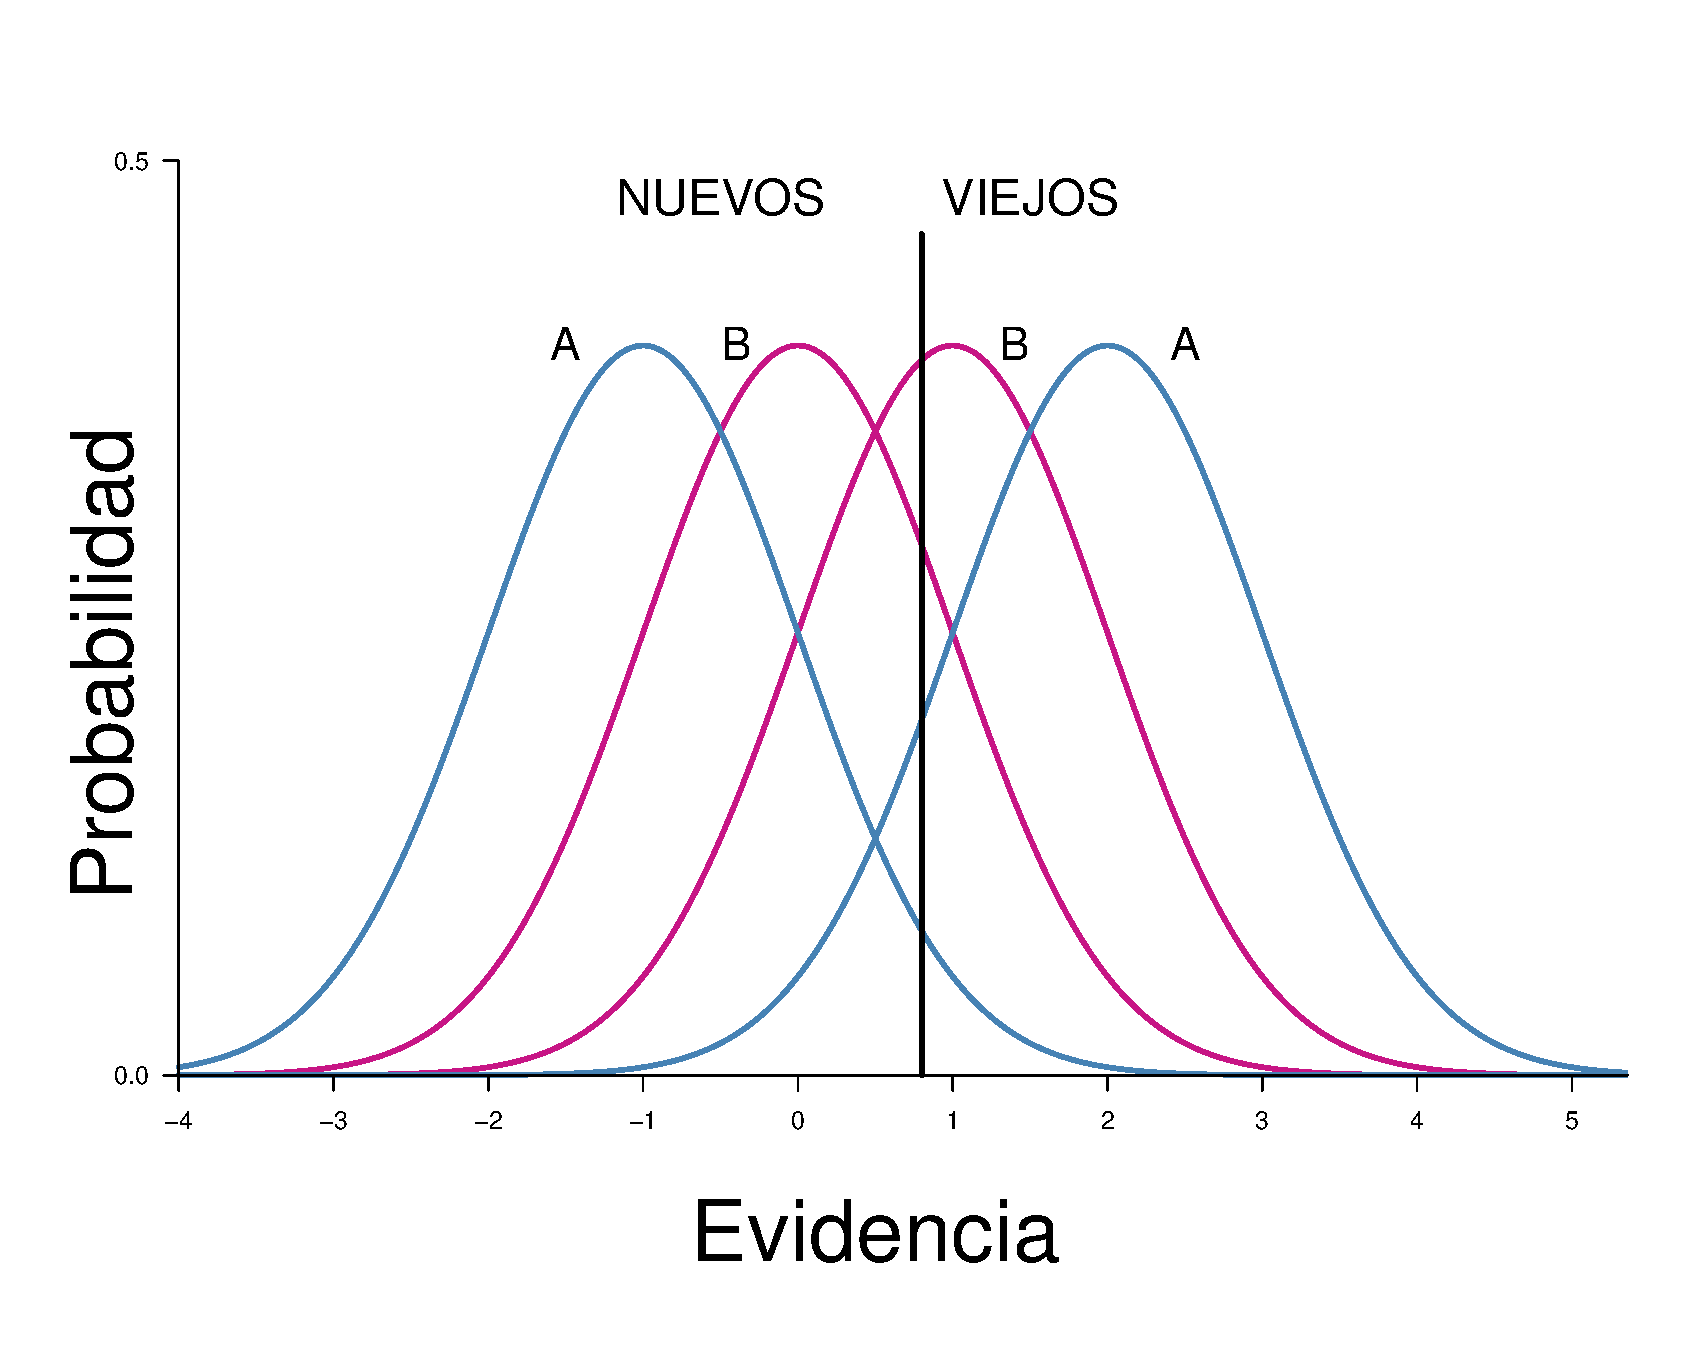
\includegraphics[width=0.7\textwidth]{Figures/EfectoEspejo_YesNo}
%\decoRule
\caption[Representación gráfica del Efecto Espejo de acuerdo a los datos obtenidos en Tareas Sí/No]{Interpretación del patrón de respuestas reportado consistentemente en tareas de reconocimiento Sí/No donde se presenta más de una clase de estímulos, con distintos niveles de $d'$. Asumiendo que el participante responde con base en un sólo criterio de elección, las tasas de Hits y Falsas Alarmas reportadas para las clases A y B sugieren que las distribuciones Señal A y B se presentan en un órden que \textit{refleja} la posición de las distribuciones de Ruido involucradas.}
\label{fig:Ejem_Espejo_YesNo}
\end{figure}

El patrón de respuestas identificado en este tipo de tareas sugiere que las cuatro distribuciones se despliegan sobre el eje de evidencia tal y como se muestra en la Figura~\ref{fig:Ejem_Espejo_YesNo}. Tomando la SDT como marco de referencia, las tasas reportadas de Falsas Alarmas y Hits para las clases A y B reflejan el área de las distribuciones de estímulos Nuevos y Viejos A y B que caen por encima del criterio, respectivamente. La figura presenta un ejemplo ideal, donde las distribuciones Nuevas no sólo reflejan el órden de las distribuciones Viejas, sino que también mantienen la misma distancia entre sí.\\

\item \underline{Efecto Espejo con Escalas de Confianza}\\

En estudios de Memoria de Reconocimiento donde se comparan los puntajes de confianza emitidos entre dos clases de estímulos A y B, se encuentra la siguiente relación en términos de los puntajes promedio asignados a cada  subconjunto de estímulos:\\

\begin{center}
$P(NuevoA) < P(NuevoB) < P(ViejoB) < P(ViejoA)$\\
\end{center}
\begin{center}
donde $P$ es el puntaje promedio asignado a los estímulos Nuevos y Viejos de cada clase de estímulo $A y B$, dentro de una Escala de Confianza donde los valores más altos señalan una mayor confianza en el juicio \textit{Viejo} y los valores más bajos, en \textit{Nuevo}, \parencite{Glanzer1993}.\\
\end{center}

De la misma forma que en su interpretación clásica, \parencite{McNicol2, McNicol5}, se asume que la asignación de cada puntaje de confianza registrado en estos experimentos está condicionada al uso de múltiples criterios de elección distribuidos sobre el eje de decisión, que van a determinar qué puntaje corresponde a cada estímulo evaluado en función a la evidencia evaluada -el punto $x$ sobre el eje de la evidencia que represente su \textit{fuerza de memoria}- y cuál sea el último criterio que esta sobrepase, (ver Figura~\ref{fig:Ejem_Efecto_Punt}).\\

\begin{figure}[th]
\centering
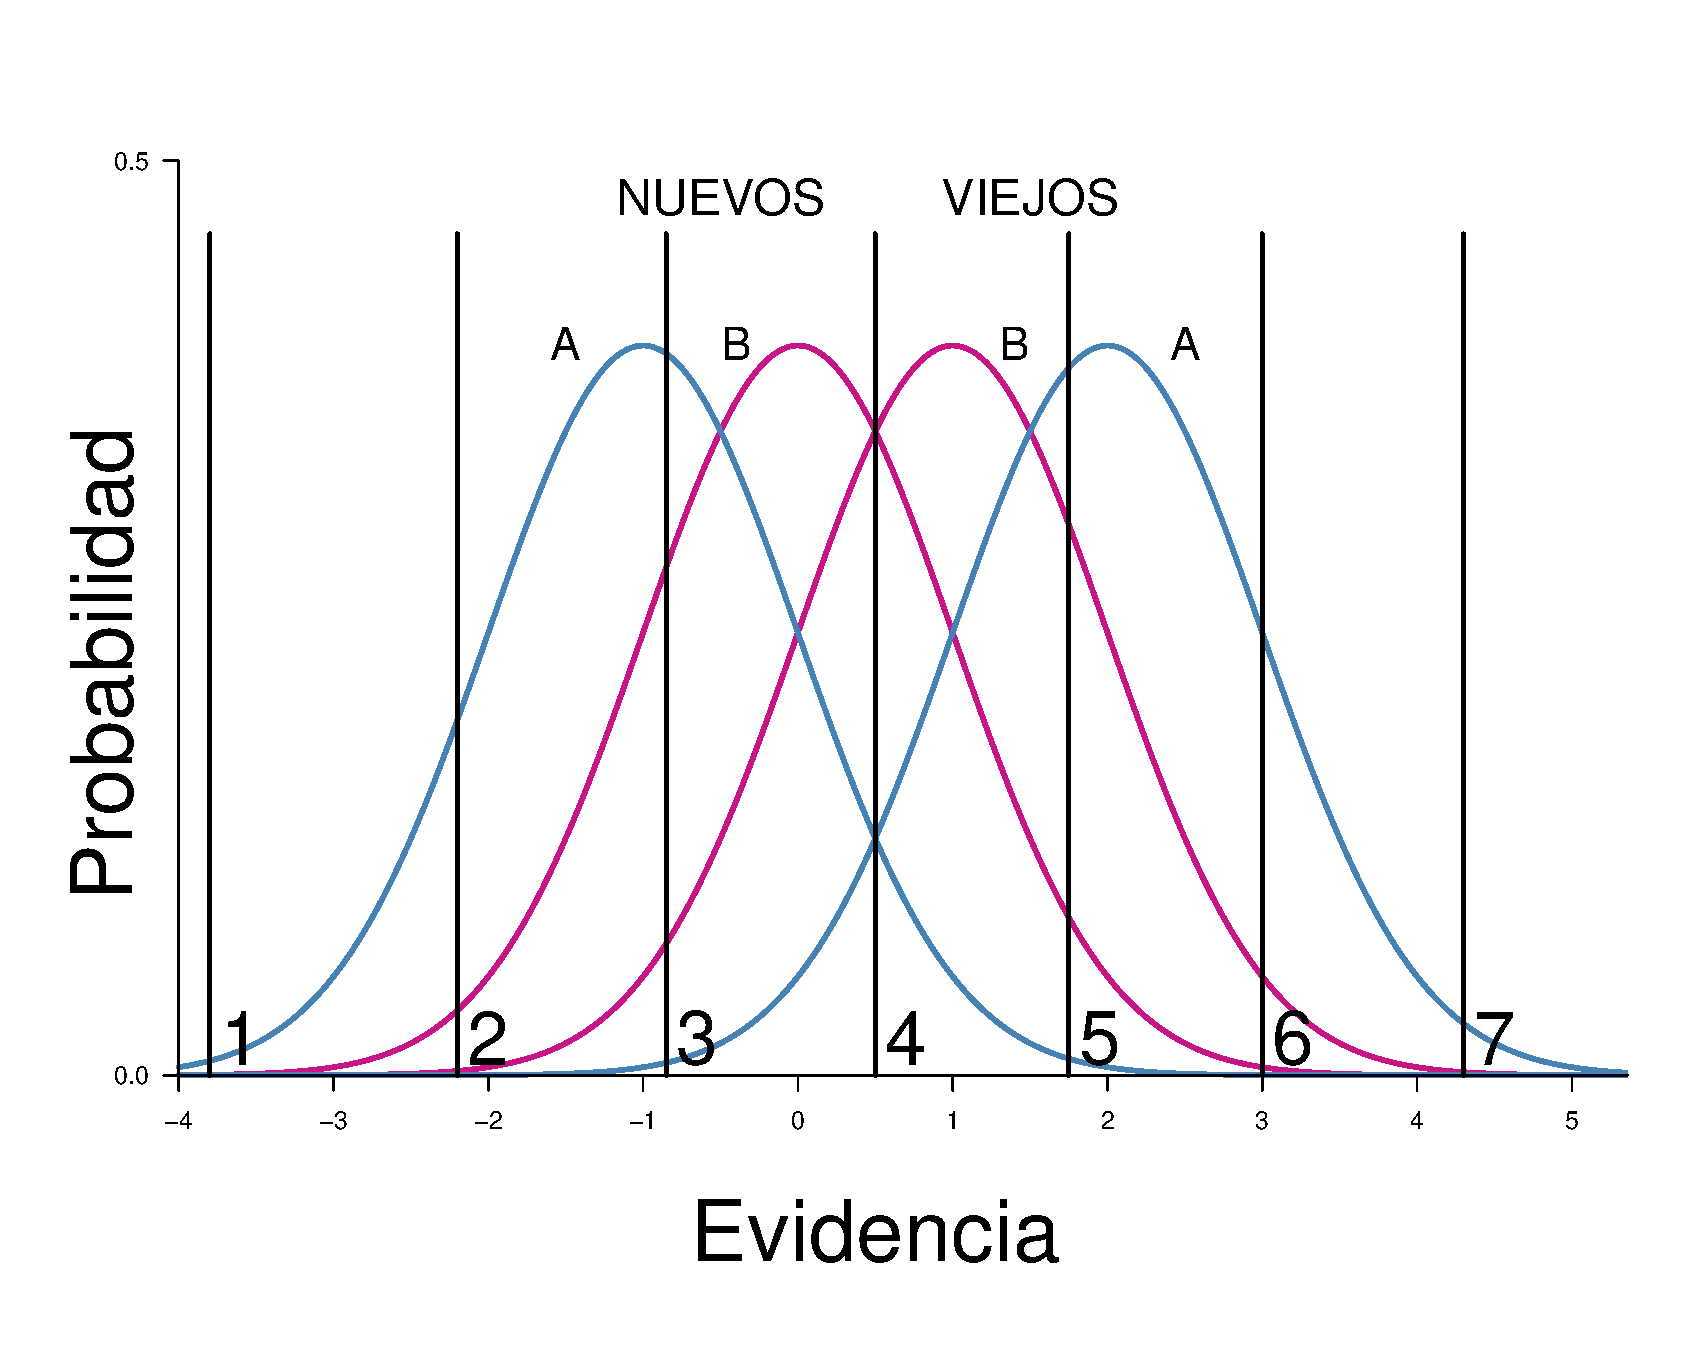
\includegraphics[width=0.7\textwidth]{Figures/EfectoEspejo_Puntajes}
%\decoRule
\caption[Representación gráfica del Efecto Espejo, de acuerdo con el patrón de respuestas registrado en tareas con Escala de Confianza]{Interpretación del patrón de respuestas reportado en tareas con Escala de Confianza en Memoria de Reconocimiento con más de una clase de estímulos. Asumiendo que el participante responde con base en los mismos sub-criterios de elección, el promedio de los puntajes asignados a cada subconjunto de estímulos aportan evidencia sobre la consistencia del Efecto Espejo como una regularidad en este tipo de tareas.}
\label{fig:Ejem_Efecto_Punt}
\end{figure}

En la Figura~\ref{fig:Ejem_Efecto_Punt} se ilustra la relación entre el promedio de los puntajes asignados a cada subconjunto de estímulos (Viejo o Nuevo x A o B) y el órden en que las cuatro distribuciones parecen desplegarse sobre el eje de evidencia. En otras palabras, que en general las distribuciones de la clase A abarcan los valores más extremos del eje de evidencia y en consecuencia, también reciben los puntajes más extremos en promedio.\\

\item \underline{Efecto Espejo en Tareas de Elección forzada entre dos alternativas}\\

Como se mencionó previamente, en las Tareas de Elección forzada de $m$ Alternativas se presenta a los participantes en cada ensayo un número $m$ de estímulos, de los cuales $m-1$ contienen Ruido y sólamente $1$, la Señal.\\

En el caso particular de los estudios en Memoria de Reconocimiento que proporcionan evidencia sobre la prevalencia y consistencia del Efecto Espejo, se refieren tareas de Elección Forzada de 2 alternativas. En dichos experimentos, se presenta a los participantes varias parejas conformadas por uno de los posibles estímulos con Señal ($ViejoA$ o $ViejoB$) y uno con Ruido ($NuevoA$ o $NuevoB$), siendo su tarea elegir cuál de estos dos estímulos le fue presentado durante la fase de estudio. De tal forma que en este tipo de estudios hay cuatro posibles tipos de parejas a presentar a los participantes en cada ensayo, (las \textit{parejas de comparación estándar}):\\

\begin{itemize}
\item Señal A VS Ruido A  (o ViejoA VS NuevoA)\\
\item Señal A VS Ruido B (o ViejoA VS NuevoB)\\
\item Señal B VS Ruido A (o ViejoB VS NuevoA)\\
\item Señal B VS Ruido B (o ViejoB VS NuevoB)\\
\end{itemize}

En tareas de elección forzada entre 2 alternativas donde se incluyen las parejas de comparación estándar ya descritas, la evidencia a favor del Efecto Espejo se reporta a partir de las siguientes relaciones:\\

\begin{center}
$P(ViejoB, NuevoB) < P(ViejoB,NuevoA)$\\
y\\
$P(ViejoA, NuevoB) < P(ViejoA,NuevoA)$\\
\end{center}
\begin{center}
donde $P$ implica la proporción de veces que el primer elemento de cada paréntesis es elegido sobre el segundo, cuando se solicita a los participantes que señalen el estímulo que se les haya presentado en la fase de estudio, \parencite{Glanzer1993}.\\
\end{center}

Al interpretar los datos obtenidos en este tipo de tareas se asume que los participantes responden en cada ensayo eligiendo el estímulo con el valor más alto, en términos de su ubicación sobre el eje de decisión. Las parejas de comparación estándar formadas en experimentos que presentan evidencia a favor del Efecto Espejo están compuestas por un estímulo extraído de alguna de las distribuciones de estímulos Viejos y un estímulo proveniente de una distribución de estímulos Nuevos. De acuerdo con la representación gráfica de la localización de las cuatro distribuciones (ver Figura~\ref{fig:Ejem_EfectoEspejo}), existe una mayor distancia entre la distribución de estímulos Nuevos A (la distribución en el extremo izquierdo) y cualquiera de las dos distribuciones de estímulos Viejos, que entre estas y la distribución de estímulos Nuevos B (la segunda distribución de izquierda a derecha). Así, el patrón de respuestas reportado en este tipo de estudios hace sentido a la luz del orden en que se despliegan las cuatro distribuciones subyacentes: los participantes aciertan en mayor proporción -pues eligen el estímulo Viejo- en las parejas compuestas por un estímulo Nuevo A, ya que la distribución correspondiente se encuentra más alejada -y es por tanto, más discriminable- de las distribuciones de estímulos Viejos.\\

Como un control adicional, en este tipo de experimentos se incluyen dos parejas adicionales (denominadas \textit{parejas de comparación nula}), que se componen por estímulos A y B, del mismo mismo tipo:\\

\begin{itemize}
\item Señal A VS Señal B (o ViejoA VS ViejoB)\\
\item Ruido A VS Ruido B (o NuevoA VS NuevoB)\\
\end{itemize}

Mientras que en las elecciones observadas entre las parejas de comparación estándar se interpretan en términos de las distancias entre las distribuciones de estímulos Viejos y las distribuciones de estímulos Nuevos, las parejas de comparación nula proporcionan información acerca de la separación entre las distribuciones del mismo tipo de ensayo, pero diferente clase de estímulo. Si las respuestas de los participantes son consistentes con la representación gráfica del Efecto Espejo, se espera encontrar que:\\

\begin{center}
$P(ViejoA, ViejoB) > 0.5$\\
y\\
$P(NuevoB, NuevoA) > 0.5$\\
\end{center}
\begin{center}
donde nuevamente $P$ representa la proporción de veces que se eligió el primer elemento de cada paréntesis como aquel que fue presentado anteriormente y $0.5$ señala la proporción que se esperaría encontrar si se asumiera que los participantes responden al azar, \parencite{Glanzer1993}.\\ 
\end{center}

El punto clave detrás de la interpretación de las elecciones observadas en las parejas de comparación nula es que están compuestas por dos estímulos que representan el mismo estado -que al elegir cualquiera de estos el participante estaría cometiendo el mismo tipo de acierto o error- y, que en teoría, deberían ser elegidos por los participantes con la misma probabilidad (con proporciones cercanas al azar, $0.5$). Sin embargo, si la representación gráfica del Efecto Espejo es un reflejo apropiado de la ejecución de los participantes en este tipo de tareas, se espera encontrar una preferencia hacia la elección de los estímulos que provengan de la distribución más orientada hacia la derecha sobre el eje de evidencia. Por ejemplo, en el caso de las parejas de comparación nula compuestas por dos estímulos Nuevos A y B, se espera que los participantes elijan con una proporción superior al azar a los estímulos B, puesto que provienen de una distribución que cubre valores más altos sobre el eje de la evidencia que la distribución Nuevos A, \parencite{Glanzer1993}.\\

\end{itemize}

En un inicio, los patrones de respuestas actualmente identificados como Efecto Espejo fueron reportados bajo el nombre de Efecto de Frecuencia de las Palabras \parencite{Schulman1967}, ya que se encontraron por primera vez en estudios donde el desempeño de los participantes en tareas de reconocimiento era comparado entre dos clases de estímulos compuestas por palabras \textit{poco comúnes} y palabras \textit{muy comunes}, de acuerdo a la Frecuencia de su uso \parencite{Kucera1967}. Dichos estudios, realizados con diferentes protocolos experimentales \parencite{Glanzer1976, Bowles1983, Glanzer1990}, demostraron consistentemente que las palabras poco comúnes eran reconocidas con mayor precisión, tanto como Nuevas como Viejas (clase A), y que las palabras comúnes se confundían con mayor facilidad (clase B). No fue hasta que se demostró que los mismos patrones de respuesta aparecían cuando dichas clases eran construidas a través de una gran variedad de manipulaciones, que se comenzó a hablar del Efecto Espejo como una regularidad más general, propia de la Memoria de Reconocimiento, \parencite{Allen1968, Glanzer1993}.\\

Hasta el día de hoy, la evidencia del Efecto Espejo ha sido reportada en una amplia variedad de estudios que definen las clases A y B de manera distinta. Por ejemplo, manipulando variables tales como la complejidad, la ortografía o la veracidad de los enunciados presentados, o bien, presentando estímulos de naturaleza diversa que se sabe influye en la precisión con que se les reconoce, como por ejemplo, palabras con significado concreto (A) vs abstracto (B), imágenes (B) vs palabras (A) o rostros comúnes (B) vs rostros poco comúnes (A), \parencite{Glanzer1993, Greene1996, Glanzer1998}.\\

\subsection{Relevancia, implicaciones e interpretaciones}\\

A primera vista, el patrón de respuestas identificado como Efecto Espejo podría parecer trivial: si sabemos que la principal diferencia entre las clases de estímulos presentadas en este tipo de estudios es la precisión con que sus elementos son reconocidos al presentarse más de una vez -es decir, que en una condición los elementos vistos se vuelven más reconocibles que en la otra-, tiene sentido esperar que los participantes tengan un mejor desempeño general (más aciertos y menos errores) en la clase A. Sin embargo, en el contexto específico del estudio de la Memoria de Reconicimiento no parece claro por qué debería haber una diferencia entre las Falsas Alarmas registradas para cada clase de estímulo, en tanto que se trata de elementos que no han sido presentados y deberían resultar igualmente \textit{familiares} -o a efectos prácticos, \textit{desconocidos}-.\\

Existen dos grandes formas en que el Efecto Espejo ha sido tratado en la literatura en Memoria de Reconocimiento:\\

\begin{enumerate}
\item Como reflejo de procesos cognitivos que subyacen a la ejecución de los participantes en tareas de reconocimiento (tanto en la fase de estudio, como en la fase de reconocimiento).\\

\item Como evidencia de que los modelos de memoria derivados de la SDT no describen adecuadamente el actuar de los mecanismos involucrados en la Memoria de Reconocimiento.\\
\end{enumerate}

Dentro de los modelos y teorías desarrollados para dar cuenta de lo que el Efecto Espejo podría estar sugiriendo acerca del funcionamiento de la Memoria de Reconocimiento se distinguen varias aproximaciones.\\

Una primera aproximación para explicar el Efecto Espejo -y probablemente la más sencilla de todas- apela a las estrategias de respuesta empleadas por los participantes. Este tipo de explicaciones se sustentan en el hecho de que las discrepancias entre las tasas de Falsas Alarmas desaparecen cuando se solicita explícitamente a los participantes que \textit{no adivinen} su respuesta \parencite{Greene1996}.\\

Por ejemplo, la hipótesis de Distribución de las Respuestas supone que los participantes asumen por \textit{default} que la cantidad de estímulos Viejos y Nuevos a presentárseles durante el experimento es la misma y en consecuencia, modulan deliberadamente la cantidad de respuestas afirmativas que emiten. Este tipo de explicaciones implican también que los participantes pueden distinguir entre las dos clases de estímulos presentadas, de forma que, dado que los elementos Viejos de la clase A se identifican con mayor precisión ($Hits(A) > Hits(B)$), \textit{acumulan} una cantidad grande de respuestas afirmativas que compensan restringiendo la emisión de juicios afirmativos en los ensayos donde la Señal está ausente y se les muestra estímulos Nuevos de la misma clase, reduciendo en consecuencia la tasa de Falsas Alarmas registrada para la clase A ($F.Alarmas(A) > F.Alarmas(B)$), \parencite{Greene1996}.\\

Un problema evidente con esta primera aproximación es que viola uno de los elementos clave detrás de la interpretación del Efecto Espejo como una fenómeno significativo y consistente en Memoria de Reconocimiento: el supuesto de que los participantes responden a partir de un sólo conjunto de criterios de elección que utilizan indistintamente entre los estímulos de clase A o B. En otras palabras, este tipo de explicaciones sólo permitirían dar cuenta de experimentos donde las clases A y B son fáciles de distinguir entre sí y dejan fuera el resto de los experimentos en que se ha encontrado evidencia del Efecto Espejo, sin que los participantes sepan que están siendo evaluados a traves de más de una clase de estímulos, \parencite{Glanzer1998}.\\

Una segunda aproximación implica asumir que las clases de estímulos empleadas en estos estudios difieren en el efecto que tienen sobre los procesos superiores involucrados en las tareas de reconocimiento. En otras palabras, este segundo conjunto de explicaciones asume que cada clase de estímulos A y B es procesada de manera diferencial por el participante. Como uno de los ejemplos más representativos de este tipo de explicaciones se encuentra la Teoría de Atención/Verosimilitud \parencite{Glanzer1993}. Dicha teoría funciona como un modelo de muestreo de rasgos que se asume que todos los estímulos a presentar están compuestos por un número fijo de rasgos ($N$), de los cuales, algunos se presentan \textit{marcados} desde su primera aparición como \textit{rasgos familiares} ($p(new)$) y otros son marcados como tales una vez que se interactúa con ellos ($p(new) + [\alpha(i)* (1-p(new))]$). Esta teoría asume que la diferencia fundamental entre  las clases de estímulos probadas ($i$) es que elicitan distintos gradientes de atención que van a repercutir en el número de rasgos atendidos por los participantes ($n(i)$) dentro de $N$, definiendo una \textit{tasa de marcaje} propia de cada clase ($\alpha(i)$).\\

En otras palabras, el proceso mediante el cual se explica el Efecto Espejo de acuerdo a la Teoría de Atención/Verosimilitud es el siguiente:\\

\begin{enumerate}
\item Todos los estímulos están compuestos por una cantidad $N$ de rasgos que pueden o no estar marcados como \textit{'conocidos'}.\\

\item Todos los estímulos comienzan con una cierta proporción de rasgos marcados.\\
\begin{center}
$p(A,nuevo) = p(new)$\\
$p(B,nuevo) = p(new)$\\
Según el modelo, la cantidad de rasgos marcados inicialmente es la misma entre las clases A y B.\\
\end{center}

\item A y B difieren en el número de rasgos que los participantes muestrean al interactuar con cada estímulo.\\
\begin{center}
$n(A) > n(B)$\\
La clase A es más atendida que B.\\
\end{center}

\item De acuerdo con $n(i)$, A y B tienen su propia tasa de muestreo.\\
\begin{center}
$\alpha(A) = \frac{n(A)}{N}$\\
$\alpha(B) = \frac{n(B)}{N}$\\
donde si $n(A) > n(B)$ entonces, $\alpha(A) > \alpha(B)$\
\end{center}

\item Al interactuar con los estímulos presentados en la fase de estudio, los participantes muestrean cierto número de rasgos y marcan aquellos que no lo estén con anterioridad, ($\alpha(i)*(1-p(new))$).\\

\item En la fase de reconocimiento, los estímulos presentados previamente tienen una mayor proporción de rasgos marcados que los estímulos nuevos:\\
\begin{center}
$p(A,viejo) = p(new) + [\alpha(A)*(1-p(new))]$\\
$p(B,viejo) = p (new) + [\alpha(B)*(1-p(new))]$\\
\end{center}
\end{enumerate}

De acuerdo con la Teoría de Atención/Verosimilitud, los participantes registran sus respuestas en la fase de reconocimiento con base en la cantidad de rasgos \textit{marcados} muestreado ($x$). La probabilidad de observar cierto valor de $x$ se describe en función a una distribución binomial con probabilidad $p(i,j)$ (donde $i$ es la clase A o B y $j$ es el tipo de estímulo: nuevo o viejos), para el total de observaciones $n(i)$ registradas en función a la clase del estímulo. Es decir:\\

\begin{center}
$p(x|p(i,j),n(i))$\\
\end{center}

Al observar una cantidad $x$ de rasgos marcados, los participantes emiten el juicio de reconocimiento que corresponda a dicha evidencia con mayor probabilidad, computando la razón de las verosimilitudes \parencite{Glanzer1993, Hintzman1994, Glanzer2009, Hilford2015}. De acuerdo con esta teoría, el Efecto Espejo se explica por medio de la siguiente relación:\\

\begin{center}
$p(x|p(A,nuevo),n(A)) < p(x|p(B,nuevo),n(B)) < p(x|p(B,viejo),n(B)) < p(x|p(A,viejo),n(A))$\\
\end{center}

En la Teoría de Atención/Verosimilitud el elemento clave para explicar las diferencias en el desempeño de los participantes entre A y B es la atención elicitada por cada clase y el número de rasgos muestreados en consecuencia ($n(i)$). Esto resuelve el problema de las discrepancias entre las tasas de Falsas Alarmas de la siguiente forma: aunque A y B contienen el mismo número de rasgos marcados en su primera presentación ($p(A,nuevo) = p(B,nuevo)$), el número de elementos muestreados es mayor en la condición A ($n(A) > n(B)$) y por tanto, hay una mayor probabilidad de extraer más rasgos marcados que en B ($p(x|p(A,nuevo),n(A)) < p(x|p(B,nuevo),n(B))$).\\

Pese al conjunto de experimentos desarrollados para probar la solidez de la Teoría de Atención/Verosimilitud mediante la manipulación de distintas variables experimentales que deberian tener un impacto sobre los parámetros del modelo (por ejemplo, restringiendo el tiempo de estudio y/o de respuesta para modificar $n(i)$ en cada fase) y evaluando la precisión con que el modelo predice y explica los datos encontrados, \parencite{Glanzer1993, Kim1993, Glanzer1991}, la Teoría de Atención/Verosimilitud ha sido fuertemente criticada en relación a dos grandes factores: 1) la teoría está compuesta por parámetros y supuestos innecesariamente complejos que le restan validez ecológica y 2) la teoría asume que los participantes tienen acceso a información completa sobre la estructura de la tarea y son capaces de utilizarla para realizar cómputos altamente demandantes, \parencite{Hintzman1994, Murdock1998, DeCarlo2007}.\\

Una tercera forma de interpretar el Efecto Espejo es de manera consistente con la aplicación de la SDT al análisis de las tareas de reconocimiento: asumiendo que los participantes registran sus respuestas en función a la evidencia que evalúan en cada ensayo (\textit{la fuerza de memoria} o \textit{familiaridad} contenida en el eje de evidencia), sin necesidad de recurrir a ningún tipo de cómputo adicional \parencite{Hintzman1994}. Bajo esta perspectiva, la única diferencia que existe entre las clases A y B -sin importar si pueda justificarse el por qué de ella- es la \textit{fuerza de memoria} que contienen, o bien qué tan familiares resultan para los participantes. Por ejemplo, en los estudios donde se usan distintos niveles de \textit{Palabras frecuentes} para delimitar las clases de estímulos a comparar, las palabras poco comúnes parecen ser más fáciles de recordar y reconocer (A) y las palabras comúnes parecen confundirse con mayor facilidad (B). De acuerdo a este tipo de explicaciones, las palabras comúnes Nuevas (B,Nuevo) tienen un mayor grado de familiaridad que los estímulos Nuevos poco comúnes (A,Nuevo), por lo que la separación de las dos distribuciones de estímulos Nuevos tiene sentido. A su vez, dado que las palabras poco comúnes son más salientes, se asume que se les presta más atención y terminan adquiriendo un mayor nivel de familiaridad cuando se les presenta por segunda vez que las palabras comúnes, lo que termina explicando el orden en que se presentan las distribuciones de estímulos Viejos, \parencite{Glanzer1993}.\\

En una dirección distinta, se encuentran las interpretaciones del Efecto Espejo que tienden a tomarle como evidencia para desacreditar el uso de la SDT para estudiar del fenómeno de la memoria de reconocimiento. Por ejemplo, un primer conflicto evidente en la interpretación del Efecto Espejo es que no siempre parece claro por qué una de las clases de estímulos a probar debería resultar \textit{más familiar} (A) que la otra (B) desde que se presenta en la fase de estudio. Aún cuando este tipo de explicaciones se sostiene de manera intuitiva para entender los resultados encontrados en estudios donde A y B se componen de palabras poco comúnes y comúnes, cuando se intenta añadir una tercer clase C, compuesta por palabras \textit{raras}, los resultados encontrados no son consistentes con lo que la interpretación del Efecto Espejo sugeriría,  \parencite{Rao1984, Wixted1992}. En general, se esperaría que la nueva clase C añadiera dos distribuciones más sobre el eje de evidencia, que se agregarían hacia los extremos inferior y superior del mismo. Sin embargo, este no parece ser el caso.\\

Por último, como un punto intermedio se encuentran los trabajos orientados al desarrollo y evaluación de distintos modelos de detección de señales que, aunque parten de los supuestos principales de la SDT, difieren en un sentido más formal, en la naturaleza que se asume tienen las distribuciones subyacentes a la tarea. Por ejemplo, asumiendo distintos tipos de distribuciones \parencite{Glanzer1993, Glanzer2009} o bien, fomentando el abordaje del problema desde la perspectiva de los modelos de mezclas en detección de señales, \parencite{DeCarlo2002, DeCarlo2007}.\\

\section{Planteamiento del problema}

Como se describió en la sección anterior, el Efecto Espejo es un fenómeno empírico reportado en estudios de Memoria de Reconocimiento desarrollados bajo el marco de la SDT. Su consistencia a lo largo de diversos procedimientos y variables impulsó el desarrollo de distintos tipos de modelos y teorías orientados a dar cuenta de este, tanto en términos de lo que podría sugerir sobre cómo opera la Memoria de Reconocimiento, como de la evaluación del modelo de detección de señales como marco para describir la ejecución de los participantes en este tipo de tareas.\\

En contraste con la amplia variedad de propuestas desarrolladas para dar cuenta del Efecto Espejo como un fenómeno intrínseco a la Memoria de Reconocimiento, es importante señalar que dicho fenómeno no ha sido estudiado ni reportado en tareas de detección pertenecientes a otro dominio donde la SDT también sea aplicada.\\

La evaluación de la generalizabilidad del Efecto Espejo a otras áreas de aplicación de la SDT se considera relevante en tanto que 1) provería un contexto más amplio para interpretar el Efecto Espejo como una regularidad derivada de los supuestos establecidos por la SDT y no como un fenómeno particular de la Memoria de Reconocimiento y 2) permitiría evaluar la pertinencia de la aplicación del modelo de detección de señales al estudio de la memoria de reconocimiento.\\

El trabajo de tesis aquí presentado no se ocupa de revisar ni de evaluar en forma alguna las propuestas teóricas y formales desarrolladas para dar cuenta del Efecto Espejo como un fenómeno inherente a la Memoria de Reconocimiento. El objetivo del trabajo de investigación realizado es el de evaluar la existencia de los patrones de respuesta identificados como Efecto Espejo en una tarea de detección desarrollada fuera del marco de la Memoria de Reconocimiento. Para ello, se propuso trabajar con una tarea de detección meramente perceptual con dos clases de estímulos A y B, construidas con base en una revisión de la literatura para que fungieran como dos niveles de discriminabilidad.\\

